\chapter{Phân tích và thiết kế hệ thống}
\textit{Chương này trình bày quá trình phân tích, thiết kế và mô hình hóa hệ thống, bao gồm khảo sát và so sánh các công trình liên quan, phân tích yêu cầu chức năng và phi chức năng, xác định các bên liên quan và các thành phần chức năng cốt lõi, xây dựng kiến trúc tổng thể của nền tảng, đồng thời minh họa các luồng tương tác và giao diện người dùng chính của hệ thống.}

\section{Phân tích và so sánh các công trình liên quan}

\subsection{Study4}

\begin{figure}[H]
        \centering
        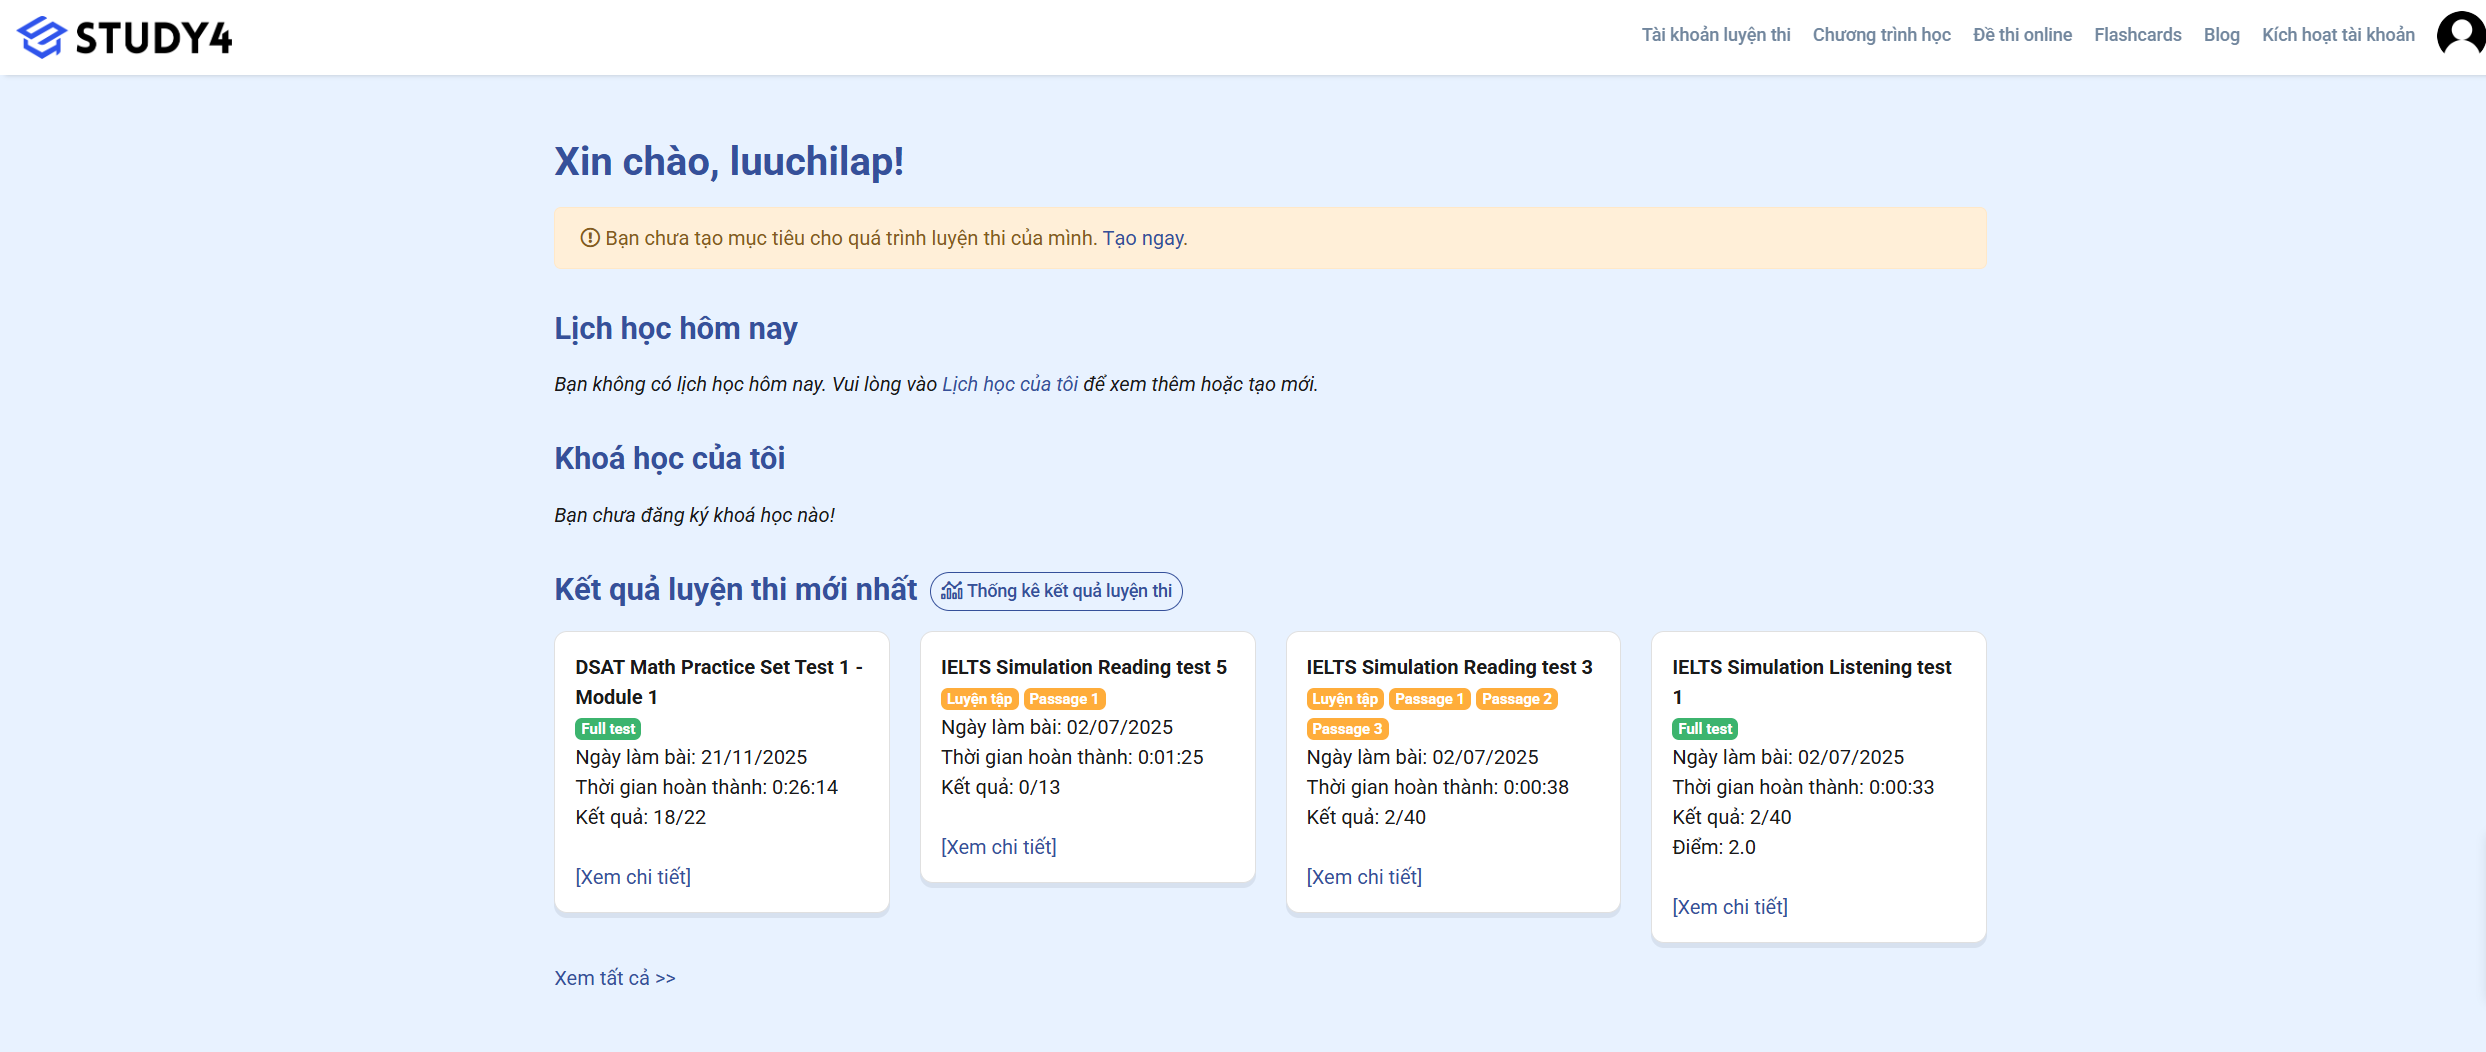
\includegraphics[width=0.7\linewidth]{graphics/related_products/study4}
        \captionsetup{skip=5pt}
        \caption{Trang chủ Study4}
\end{figure}  

Study4 là một nền tảng học tiếng Anh trực tuyến cung cấp nội dung ôn luyện cho các chứng chỉ quốc tế như IELTS, TOEIC và HSK. Nền tảng này cung cấp tài nguyên cho học viên muốn cải thiện năng lực ngôn ngữ và vượt qua các kỳ thi chuẩn hóa.

Nền tảng cung cấp nhiều tính năng nhằm nâng cao trải nghiệm học tập. Người dùng có thể lựa chọn các khóa học có thể tùy biến, bao gồm chương trình toàn diện hoặc các mô-đun chuyên biệt tập trung vào từng kỹ năng như đọc hoặc viết, giúp nền tảng phù hợp với người học ở nhiều trình độ khác nhau. Nội dung được chia thành các phần nhỏ, dễ theo dõi để hỗ trợ tiếp thu kiến thức tốt hơn. Ngoài ra, nền tảng còn tích hợp nhiều công cụ hữu ích ngay trong giao diện học tập như tra từ điển tức thời, tô sáng, ghi chú và bộ flashcard từ vựng được cập nhật, thường áp dụng kỹ thuật lặp lại ngắt quãng. Study4 cũng có hệ thống gắn thẻ phong phú, cho phép người dùng dễ dàng xem tổng hợp kết quả theo dạng câu hỏi hoặc loại kỳ thi, từ đó theo dõi tiến độ và xác định các điểm cần cải thiện.

Về ưu điểm, Study4 hỗ trợ nhiều dạng kỳ thi như IELTS, TOEIC, SAT và HSK, cho phép người dùng xem lại kết quả các bài thi trước đó và sử dụng flashcard để ôn tập từ vựng. Nền tảng sở hữu hệ thống gắn thẻ phong phú cho câu hỏi và bài thi, cung cấp các khóa học chuyên biệt và có blog để tương tác với cộng đồng người dùng. Ngoài ra, các phần giải thích kết quả có sẵn và khu vực bình luận còn khuyến khích thảo luận và nâng cao hiệu quả học tập.

Về nhược điểm, Study4 thiếu sự hướng dẫn trực tiếp từ giáo viên, chức năng tìm kiếm còn hạn chế và hiện chủ yếu chỉ phục vụ học sinh Việt Nam. Bên cạnh đó, nền tảng chưa hỗ trợ bài thi Viết và Nói, làm giảm tính hữu ích đối với nhu cầu ôn luyện toàn diện.

\subsection{IELTS Online Tests}

\begin{figure}[H]
        \centering
        
\includegraphics[width=0.7\linewidth]{graphics/related_products/ito}
        \captionsetup{skip=5pt}
        \caption{Trang chủ IELTS Online Tests}
       
\end{figure}

IELTS Online Tests cho phép thí sinh thực hiện bài thi IELTS Academic từ xa tại nhà hoặc ở một địa điểm riêng tư khác có kết nối Internet ổn định. Bài thi tuân theo cùng định dạng, nội dung và tiêu chuẩn bảo mật như bài thi trên máy tính tại trung tâm.

Bài thi đánh giá đầy đủ bốn kỹ năng tiếng Anh — Nghe, Đọc, Viết và Nói — trong khoảng 2 giờ 45 phút. Phần thi Nói được tổ chức trực tiếp qua cuộc gọi video với giám khảo được chứng nhận, giữ nguyên tính tương tác trực diện vốn là đặc trưng của IELTS. Nội dung và dạng câu hỏi hoàn toàn giống với bài thi Academic tại trung tâm.

IELTS Online vận hành trên cổng thi Inspera Exam Portal an toàn và sử dụng kết hợp giám sát bằng AI cùng giám thị từ xa để đảm bảo tính trung thực. Kết quả được trả dưới dạng điện tử trong vòng 6–8 ngày và không phát hành phiếu kết quả bản giấy. Điều kiện dự thi giới hạn cho thí sinh từ 18 tuổi trở lên; thiết bị yêu cầu là máy tính để bàn hoặc laptop có webcam, micro và loa hoạt động tốt, ưu tiên thiết bị có dây.

Về ưu điểm, IELTS Online Tests chuyên sâu vào IELTS trên cả bốn kỹ năng, cung cấp kho bài luyện tập lớn và giao diện mô phỏng rất sát môi trường thi thật. Nền tảng phục vụ học viên tại hơn 120 quốc gia, có lớp học trực tiếp ở nhiều múi giờ và cung cấp các bài kiểm tra thử với người thật, qua đó tăng tính chân thực của trải nghiệm học tập.

Về nhược điểm, IELTS Online Tests chỉ giới hạn ở kỳ thi IELTS và không hỗ trợ các kỳ thi khác. Nền tảng không có giao diện di động và tập người dùng bị giới hạn do các ràng buộc về độ tuổi, địa điểm và quốc tịch. Chi phí cao cho dịch vụ Viết và Nói khiến nền tảng khó tiếp cận hơn đối với học viên ở các nước đang phát triển; phản hồi cũng phụ thuộc vào lịch của giám khảo nên có thể bị chậm. Ngoài ra, nền tảng không có diễn đàn hay không gian thảo luận cho người học.

\subsection{The Forum}

\begin{figure}[H]
        \centering
        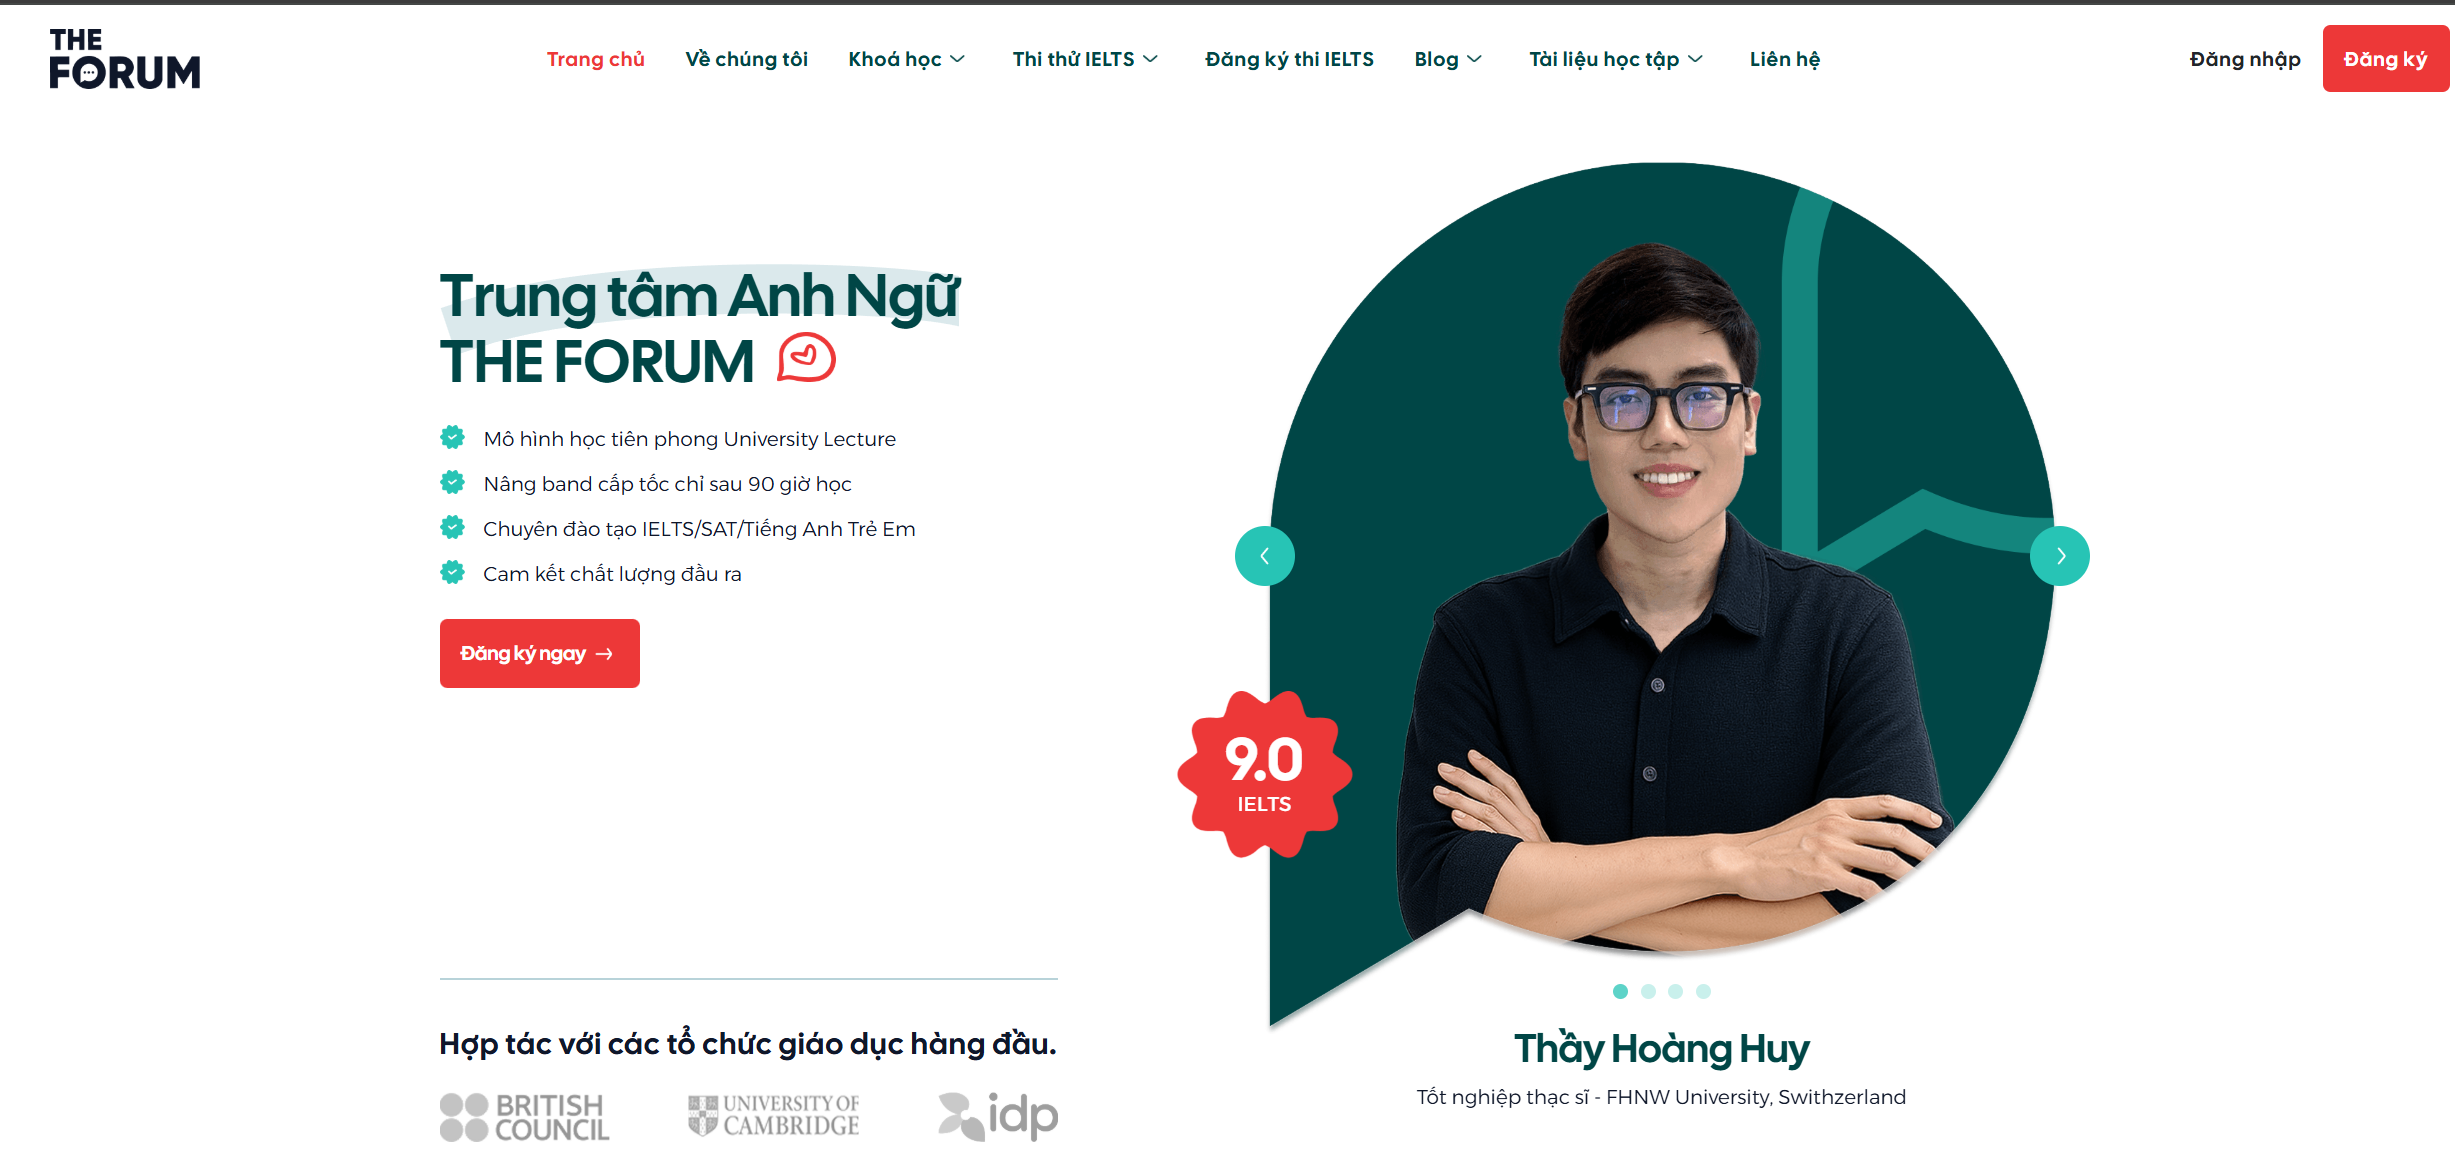
\includegraphics[width=0.7\linewidth]{graphics/related_products/forum}
        \captionsetup{skip=5pt}
        \caption{Trang chủ The Forum}
       
\end{figure}

The Forum là một tổ chức giáo dục tại Việt Nam cung cấp chương trình đào tạo tiếng Anh toàn diện và ôn luyện cho các kỳ thi IELTS và SAT. Đơn vị này triển khai cả khóa học trực tuyến lẫn trực tiếp, nhấn mạnh chất lượng giảng dạy cao thông qua đội ngũ chuyên môn và công nghệ hiện đại.

Về ưu điểm, The Forum cung cấp các buổi học trực tiếp và livestream miễn phí, có dịch vụ phản hồi cho kỹ năng Viết và Nói, đồng thời hỗ trợ cả hình thức học trực tuyến và trực tiếp. Nền tảng cũng cung cấp các bài kiểm tra thử để hỗ trợ học viên luyện tập hiệu quả.

Về nhược điểm, The Forum có lượng tài nguyên học trực tuyến công khai còn hạn chế và số lượng bài thi sẵn có chưa nhiều. Đối tượng mục tiêu chủ yếu là học viên Việt Nam nên phạm vi tiếp cận còn bị giới hạn.

\subsection{Prep Education}

\begin{figure}[H]
        \centering
        
\includegraphics[width=\linewidth]{graphics/related_products/prep}
        \captionsetup{skip=5pt}
        \caption{Trang chủ Prep Education}
       
\end{figure}

Prep Education là một nền tảng công nghệ giáo dục thế hệ mới ứng dụng AI nhằm cá nhân hóa việc học ngôn ngữ, kiểm tra và giảng dạy. Nền tảng chủ yếu phục vụ người học trên khắp châu Á, hỗ trợ họ chuẩn bị cho các kỳ thi ngôn ngữ quốc tế và cải thiện kỹ năng giao tiếp thông qua công nghệ tiên tiến cùng sự hướng dẫn của chuyên gia.

Nền tảng tận dụng trí tuệ nhân tạo và cấu trúc khóa học toàn diện để mang đến trải nghiệm học tập thích ứng và hấp dẫn. Các kế hoạch học tập cá nhân hóa được tạo ra dựa trên trình độ hiện tại và mục tiêu của người học, với các mục tiêu hằng ngày và hằng tuần rõ ràng. Người dùng có thể luyện nói trong phòng nói ảo mô phỏng điều kiện thi thật, nhận chấm điểm tức thì cùng phản hồi chi tiết về phát âm, độ trôi chảy và ngữ pháp. Tương tự, phòng viết ảo cho phép người học luyện tập các dạng bài thi với phản hồi và chấm điểm bằng AI theo các tiêu chí đánh giá chính thức, từ đó đẩy nhanh quá trình cải thiện.

Prep Education còn tích hợp Teacher Bee AI, một gia sư ảo hoạt động 24/7 có thể hỗ trợ tức thì, trả lời câu hỏi, tóm tắt bài học và tạo thêm bài tập như một người bạn đồng hành học tập cá nhân. Hệ thống chấm điểm AI độc quyền của nền tảng đưa ra phản hồi chính xác về ngữ pháp, từ vựng, tính mạch lạc, giọng điệu và phát âm. Nền tảng cung cấp đa dạng khóa học, bao gồm ôn thi IELTS, TOEIC, HSK (năng lực tiếng Trung) và tiếng Anh tổng quát cho giao tiếp hoặc công việc (PrepTalk).

Về ưu điểm, Prep Education phục vụ nhiều nhóm người học, từ người học tiếng Anh tổng quát đến thí sinh ôn thi, và có khả năng tiếp cận trên phạm vi toàn cầu. Nền tảng tích hợp AI cho các tính năng Nói và Viết, cung cấp cả lớp học trực tuyến, trực tiếp và các bài kiểm tra thử, đồng thời có giao diện thân thiện với người dùng. Hệ thống hỗ trợ nhiều định dạng kỳ thi như IELTS, TOEIC, HSK và nhiều kỳ thi khác, đồng thời có mặt trên cả website và ứng dụng di động.

Về nhược điểm, Prep Education chưa cung cấp phản hồi từ giám khảo con người cho kỹ năng Nói và Viết, và các tính năng AI vẫn có thể được phát triển sâu hơn. Ngoài ra, nền tảng còn thiếu các chức năng như “lưu không gian làm việc” hoặc “ôn tập kiến thức” dành cho học viên.

\subsection{Comparision}

Dưới đây là các kết luận chúng tôi rút ra từ việc phân tích các hệ thống trước đó.

{
\scriptsize
\setlength{\tabcolsep}{3pt}
\renewcommand{\arraystretch}{1.5}
\setlist[enumerate]{leftmargin=*, labelsep=0.5em}

\begin{tabularx}{\textwidth}{|>{\raggedright\arraybackslash}X|>{\raggedright\arraybackslash}X|>{\raggedright\arraybackslash}X|>{\raggedright\arraybackslash}X|>{\raggedright\arraybackslash}X|>{\raggedright\arraybackslash}X|>{\raggedright\arraybackslash}X|}
\hline
\textbf{Tên} & \textbf{Định dạng bài thi} & \textbf{Có dùng AI} & \textbf{Có thi Nói/Viết} & \textbf{Chi phí} & \textbf{Điểm nổi bật} & \textbf{Nền tảng} \\
\hline
Study4 & IELTS, TOEIC, SAT, HSK, v.v. & Không & Không & Miễn phí, có khóa trả phí & Flashcard và các tính năng hỗ trợ & Web và di động \\
\hline
IELTS Online Tests & IELTS & Kết hợp (giám khảo thật cho Speaking/Writing, AI cho giao diện) & Có & Trả phí & Mô phỏng thi thật; bài kiểm tra thử với người thật & Chỉ web \\
\hline
The Forum & Số lượng bài thi hạn chế; không rõ định dạng & Không & Có & Trả phí & Lớp học trực tiếp; trực tuyến hoặc trực tiếp & Web và trực tiếp \\
\hline
Prep Edu & IELTS, TOEIC, HSK, tiếng Anh tổng quát, v.v. & Có & Có & Trả phí & Lớp học trực tuyến hoặc trực tiếp; phòng luyện nói ảo & Web và ứng dụng di động \\
\hline
\caption{So sánh các nền tảng ôn thi tiếng Anh}
\end{tabularx}

}

Việc phân tích các nền tảng hiện có cho thấy, cả tại Việt Nam lẫn trên thế giới, thị trường ôn luyện tiếng Anh ứng dụng AI vẫn còn tương đối hạn chế. Mặc dù một số nền tảng đã tích hợp AI cho học tập thích ứng, chấm điểm hoặc phản hồi, phần lớn vẫn chưa khai thác hết tiềm năng của công nghệ này, đặc biệt ở các mảng như đánh giá tự động kỹ năng Nói và Viết, lập kế hoạch học tập cá nhân hóa và phân tích hiệu suất theo thời gian thực. Đây là cơ hội rõ ràng để đổi mới, đồng thời nhóm cũng có thể học hỏi từ ưu điểm và hạn chế của các nền tảng hiện có để thiết kế một giải pháp hiệu quả hơn.

Trong bối cảnh đó, tính khả thi của dự án là cao. Bằng cách tích hợp các tính năng AI tiên tiến, phạm vi hỗ trợ kỳ thi toàn diện và giao diện thân thiện với người dùng — đồng thời khắc phục những khoảng trống quan sát được ở các nền tảng khác — chúng tôi có thể xây dựng một nền tảng mang lại giá trị khác biệt cho người học tại Việt Nam cũng như quốc tế. Việc rút kinh nghiệm từ thành công và hạn chế của các giải pháp hiện tại cho phép nhóm cải tiến các cách tiếp cận sẵn có và mang lại trải nghiệm học tập tốt hơn.

\section{Phân tích yêu cầu}

\subsection{Các bên liên quan}

Việc thiết kế hệ thống hiệu quả đòi hỏi phải hiểu rõ nhu cầu và kỳ vọng của các bên liên quan. Nền tảng của chúng tôi phục vụ bốn nhóm bên liên quan chính:

\begin{itemize}
\item \textbf{Examinee/Learner (User)}: Đây là nhóm người dùng chính của nền tảng, bao gồm các thí sinh có trình độ đa dạng từ beginner đến advanced. Mục tiêu chính của họ là cải thiện điểm số thông qua quá trình luyện tập hiệu quả và personalized feedback. Nhóm người dùng này cần giao diện trực quan, tài liệu luyện tập toàn diện và các insight có thể hành động được về kết quả học tập của mình.

\item \textbf{Administrator}: Các quản trị viên nền tảng chịu trách nhiệm quản lý content, theo dõi usage pattern và bảo đảm chất lượng hệ thống. Họ cần các công cụ cho content management, user administration và analytics dashboard để hiểu được platform performance cũng như mức độ user engagement.
\end{itemize}

\subsection{Yêu cầu chức năng}
{
\renewcommand{\arraystretch}{1.5} % increase row height
\begin{tabularx}{\textwidth}{|l|l|X|}
\hline
\textbf{ID} & \textbf{Tên FR} & \textbf{Mô tả} \\ \hline
FR1 & Authentication and Authorization & Nền tảng phải triển khai cơ chế user authentication an toàn với role-based access control. Các user role bao gồm Examinee và Administrator, với các permission set riêng biệt. Guest access cần được hỗ trợ cho các tính năng công khai mà không yêu cầu authentication. \\ \hline
FR2 & Multi-Exam Support & Nền tảng phải hỗ trợ đầy đủ các định dạng bài thi cho các kỳ thi IELTS, TOEIC, TOEFL và SAT. \\ \hline
FR3 & Đánh giá Speaking & 
\begin{minipage}[t]{\linewidth}
Nền tảng phải cung cấp chức năng speaking assessment toàn diện, bao gồm:
\begin{itemize}
    \item Speech-to-text transcription sử dụng Whisper API với timestamp ở mức từng từ
    \item Pause và silence detection sử dụng librosa để phân tích fluency
    \item Phân tích intonation và pitch (F0) bằng Parselmouth để đánh giá pronunciation
    \item Aggregated scoring bám sát các tiêu chí official band score
    \item AI-generated feedback kèm các đề xuất cải thiện cụ thể
\end{itemize}
\end{minipage} \\ \hline
FR4 & Speaking Simulation & Nền tảng phải cung cấp các phiên luyện Speaking chân thực, sử dụng Whisper cho voice input, deepfake-generated examiners để tăng tính trực quan và các câu hỏi được điều chỉnh dựa trên câu trả lời của người dùng. \\ \hline
FR5 & Knowledge Management & Người dùng phải có thể tạo các bộ flashcard, lưu vocabulary và grammar item, ghi chú trong quá trình luyện tập và tổ chức tài liệu học tập thành các custom collection. \\ \hline
\caption{Bảng yêu cầu chức năng}
\end{tabularx}}



\subsection{Yêu cầu phi chức năng}

{
\renewcommand{\arraystretch}{1.5} % increase row height
\begin{tabularx}{\textwidth}{|l|l|X|}
\hline
\textbf{ID} & \textbf{Tên NFR} & \textbf{Mô tả} \\ \hline
NFR1 & Performance & Thời gian tải trang trung bình không được vượt quá 2 giây. Quá trình speaking evaluation phải hoàn tất trong vòng 20 giây kể từ khi gửi audio. API response time trung bình phải dưới 500 milliseconds đối với các thao tác non-AI. \\ \hline
NFR2 & Scalability & Nền tảng phải hỗ trợ ít nhất 10.000 concurrent user thông qua kiến trúc containerized microservices. Mỗi service phải có khả năng scale độc lập theo nhu cầu. \\ \hline
NFR3 & Availability & Nền tảng phải duy trì 99.9\% availability với các cơ chế redundancy và failsafe đa dạng. \\ \hline
NFR4 & Portability & Nền tảng phải bảo đảm hành vi nhất quán giữa các môi trường development, staging và production. \\ \hline
NFR5 & Security & Tất cả communication phải được mã hóa. Các internal module không được exposed ra bên ngoài. Các connection request phải được authenticated và authorized tùy theo permission tương ứng. User authentication phải sử dụng JWT token với thời hạn hết hạn phù hợp. Sensitive data phải được mã hóa khi lưu trữ. \\ \hline
NFR6 & Maintainability & Codebase phải tuân thủ các coding standard đã được thiết lập, bao gồm comprehensive documentation và đạt tối thiểu 80\% test coverage đối với các critical component. \\ \hline
\caption{Bảng yêu cầu phi chức năng}
\end{tabularx}
}
\section{Usecase của hệ thống}
\subsection{Tổng quan}
Các use case của hệ thống có thể được tổ chức thành ba module chính, mỗi module giải quyết một khía cạnh cốt lõi trong chức năng của nền tảng. Module thứ nhất, Authorization, Authentication, and Profile Management, bao gồm toàn bộ use case liên quan đến user registration, login, role-based access control và quản lý thông tin cá nhân. Module thứ hai, Learning Activities, bao gồm các use case về truy cập khóa học, thực hiện bài luyện tập, xem lại kết quả và tương tác với các công cụ học tập có hỗ trợ AI. Module thứ ba, Staff Activities, bao gồm các use case dành cho tác vụ quản trị, content management và monitoring.

Trong phiên bản hiện tại, phần use case chi tiết trong chương này được để trống tạm thời để phục vụ quá trình sắp xếp lại bộ use case mới. Toàn bộ use case mới hiện được đặt ở phần phụ lục, sau đó các use case chính sẽ được chọn và chuyển trở lại chương này ở bước tiếp theo.

\subsection{Sơ đồ tổng quan các module use case}

Hệ thống được chia thành hai hệ thống con chính: \textbf{Server} (hệ thống microservices phục vụ luyện thi) và \textbf{Engapp-v2} (nền tảng học tiếng Anh blended learning). Mỗi hệ thống con có bộ use case riêng biệt, được tổng hợp trong hai sơ đồ dưới đây.

\begin{figure}[H]
        \centering
        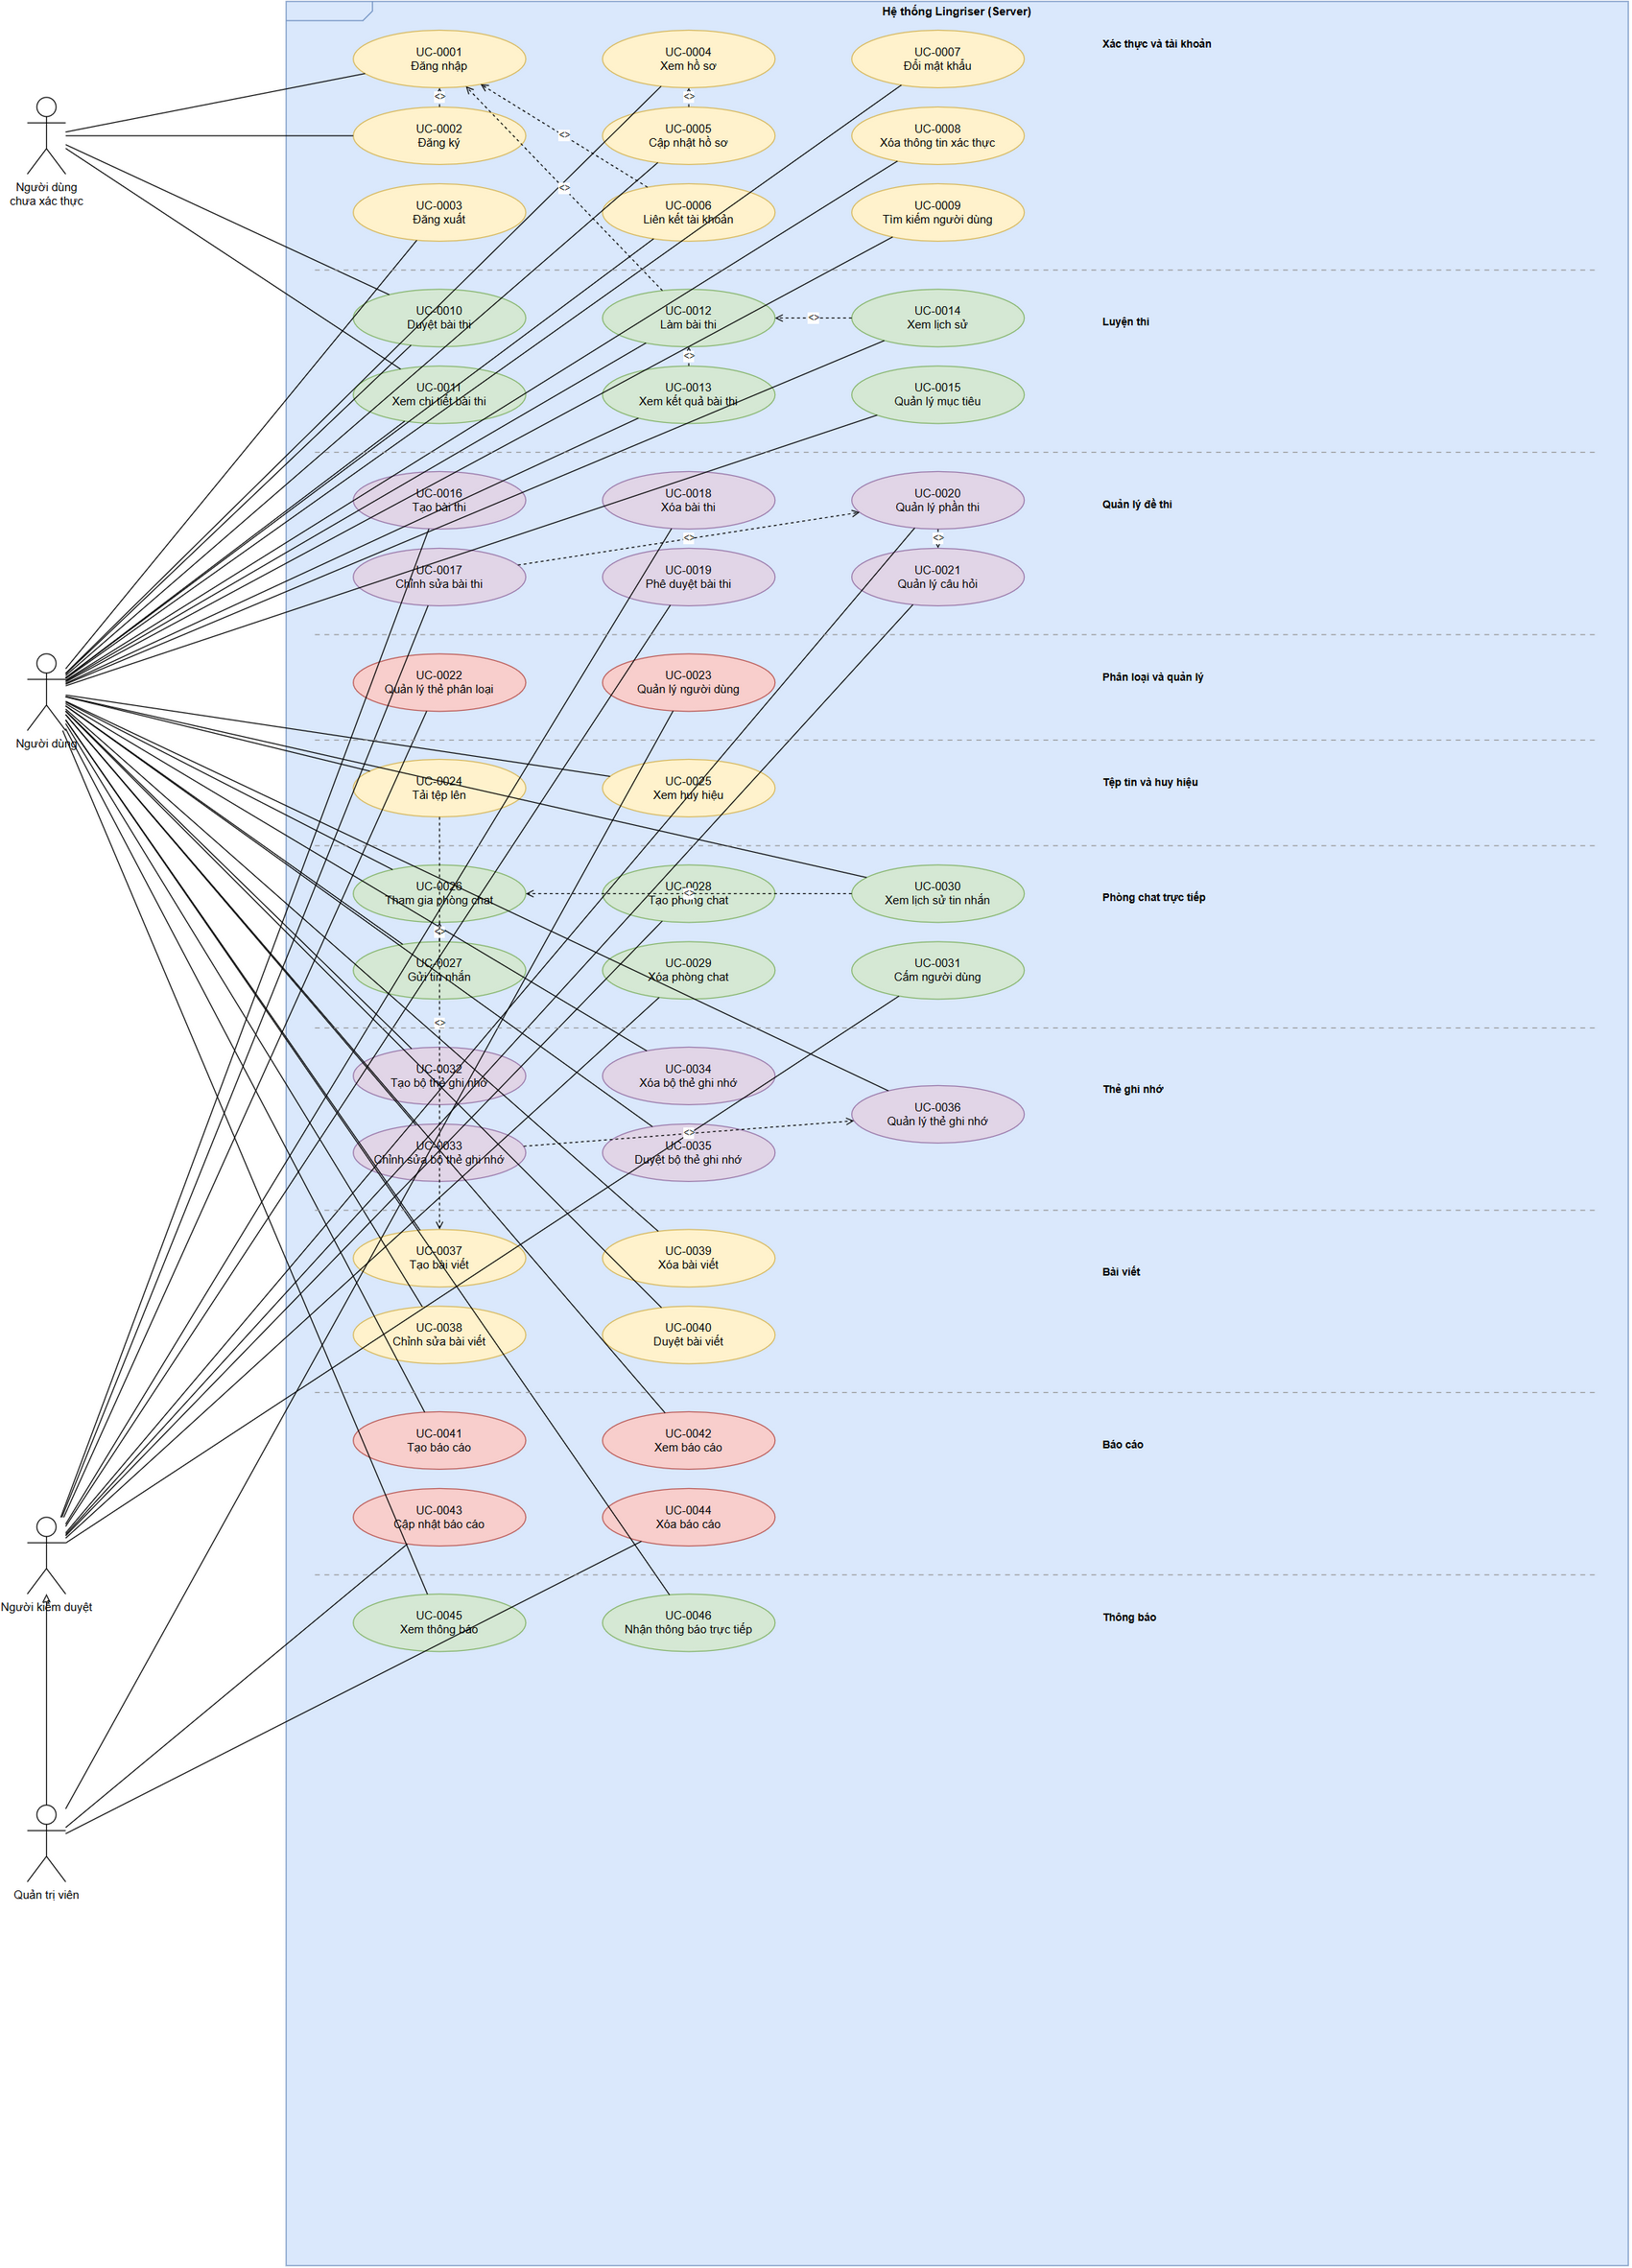
\includegraphics[width=\linewidth]{graphics/usecases/server}
        \captionsetup{skip=5pt}
        \caption{Sơ đồ Use case tổng quan --- Hệ thống Server (Microservices luyện thi)}
        \label{UCServer}
\end{figure}

Hình~\ref{UCServer} minh họa các use case của hệ thống Server, bao gồm các module: Authentication \& Account (UC-0001 đến UC-0009), Exam Practice (UC-0010 đến UC-0015), Exam Management (UC-0016 đến UC-0021), Tag Taxonomy (UC-0022), User Management (UC-0023), File Upload (UC-0024), Achievements \& Badges (UC-0025), Live Chat (UC-0026 đến UC-0031), Flashcards (UC-0032 đến UC-0036), và Blog (UC-0037 đến UC-0040).

\begin{figure}[H]
        \centering
        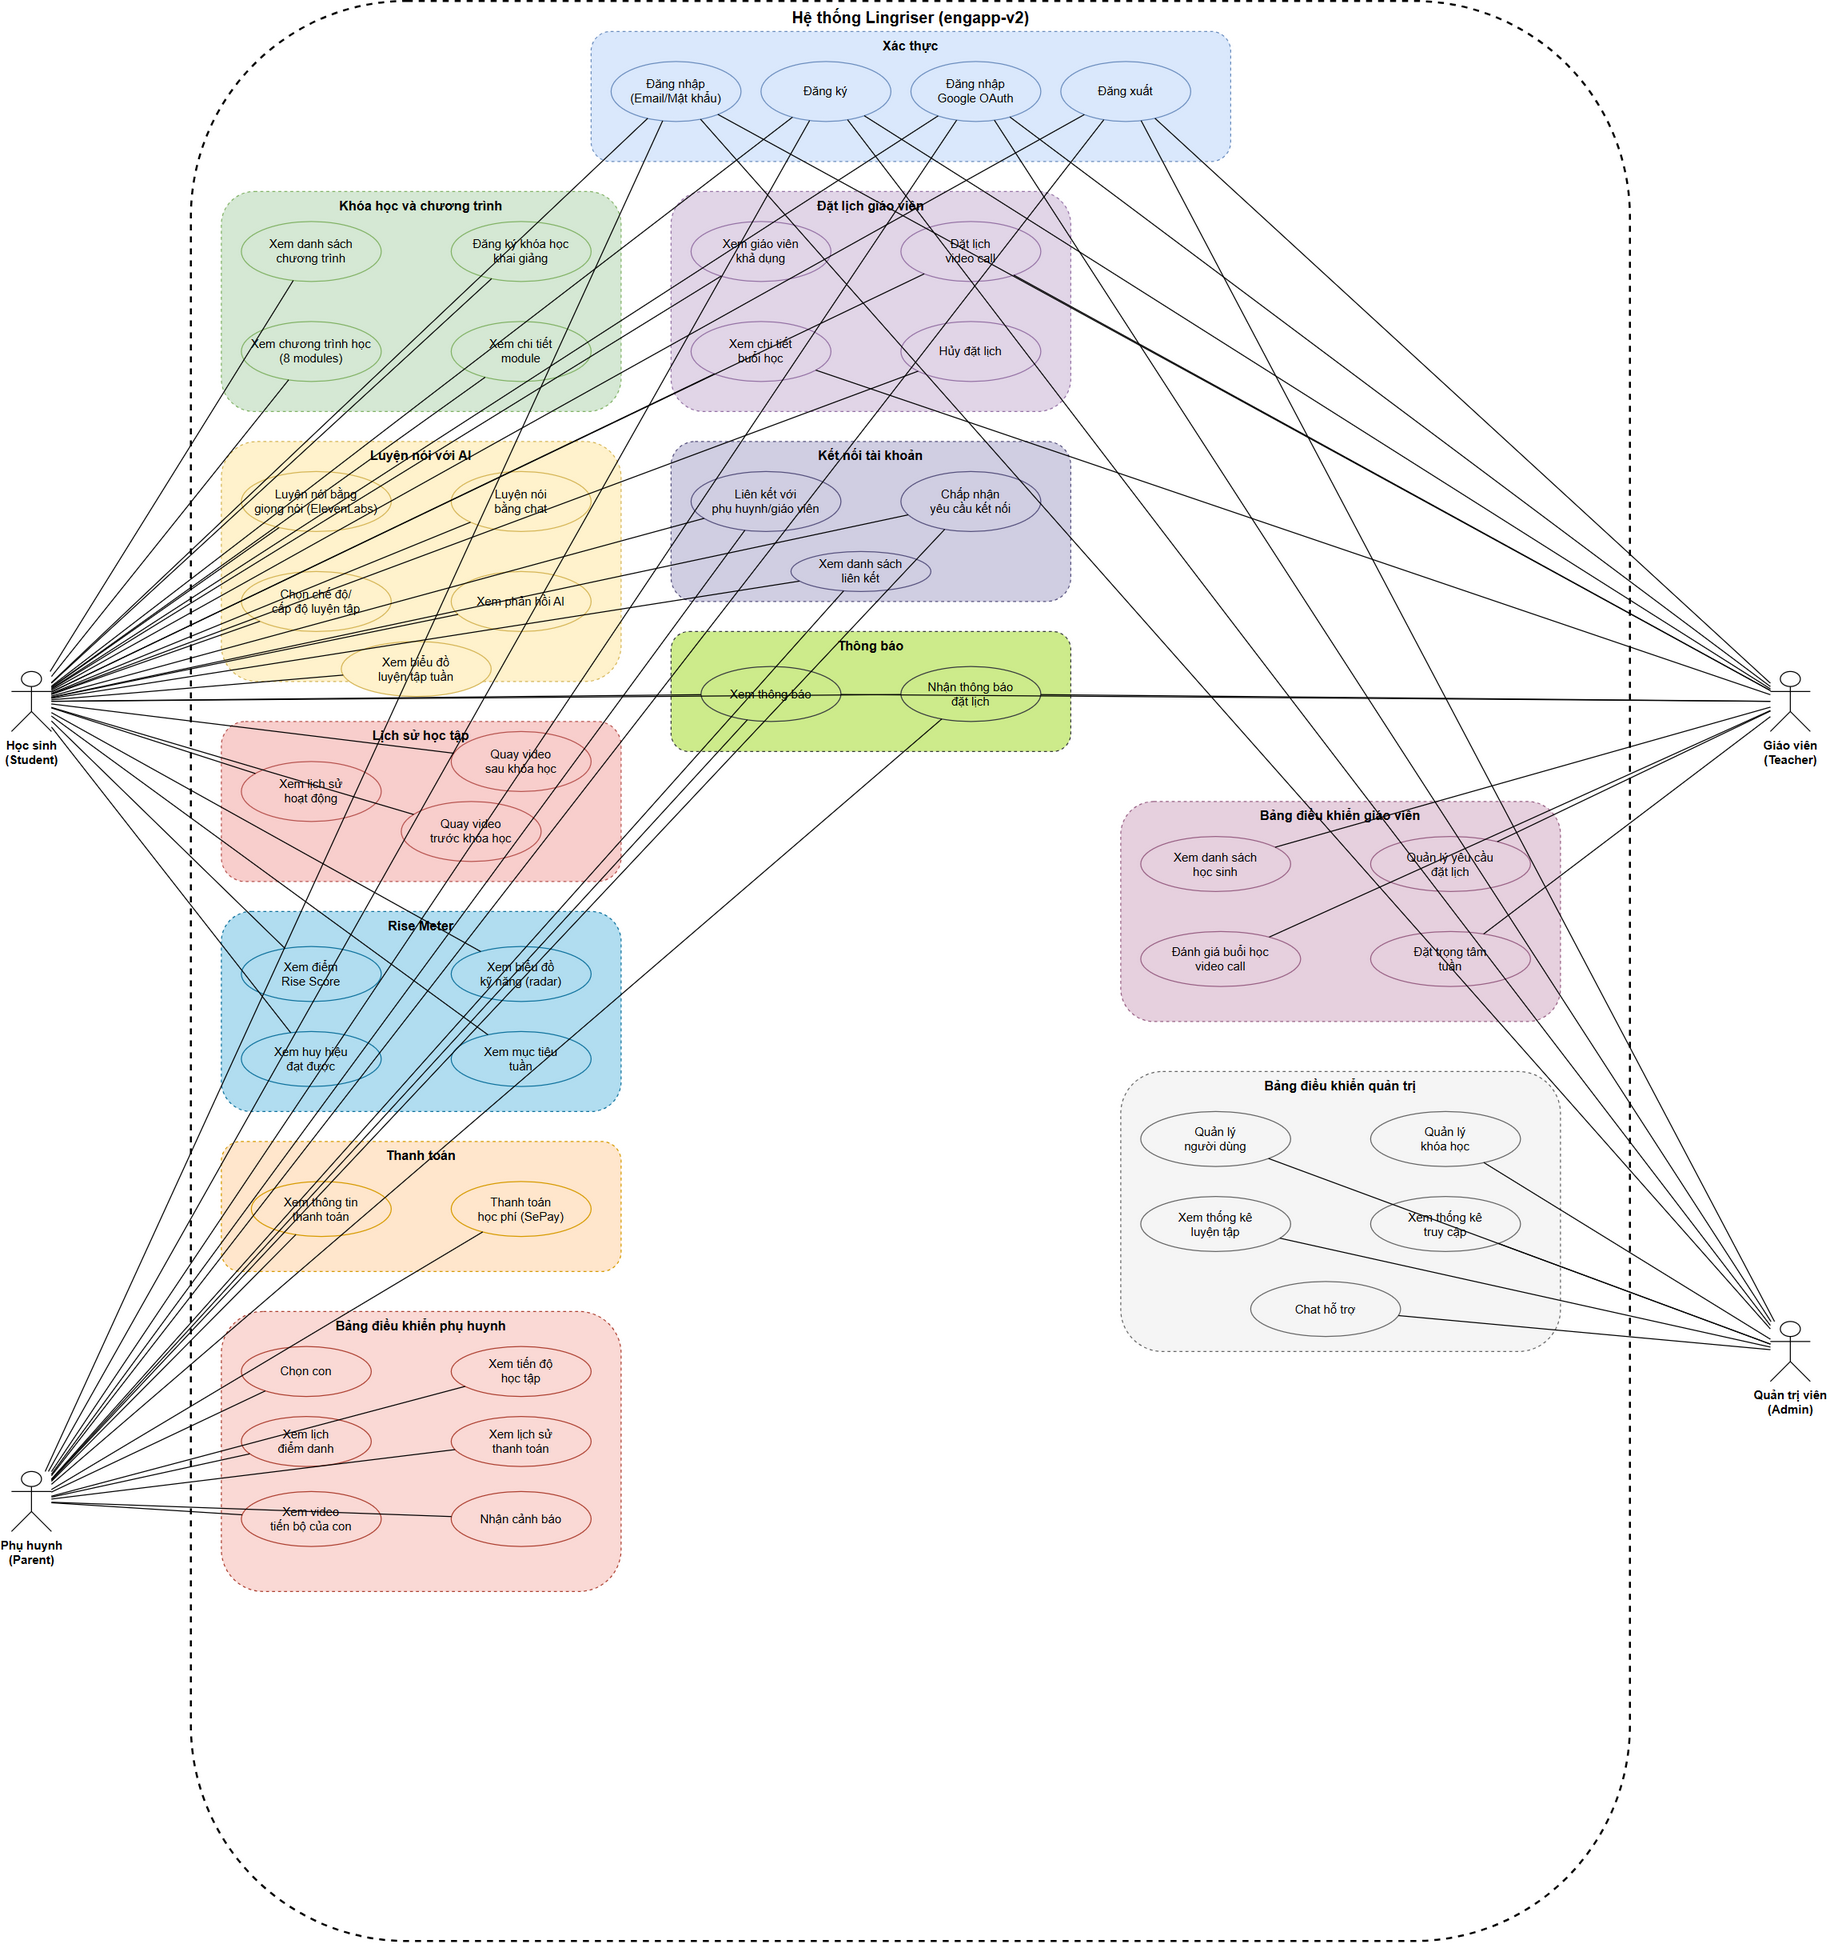
\includegraphics[width=\linewidth]{graphics/usecases/engapp-v2}
        \captionsetup{skip=5pt}
        \caption{Sơ đồ Use case tổng quan --- Nền tảng Engapp-v2 (Blended Learning)}
        \label{UCEngapp}
\end{figure}

Hình~\ref{UCEngapp} minh họa các use case của nền tảng Engapp-v2, bao gồm các module: Quản lý khóa học \& ghi danh, Đặt lịch video call với giáo viên, Luyện nói AI (ElevenLabs), Theo dõi quá trình học tập, Thanh toán (SePay), Quản lý kết nối tài khoản (học sinh -- phụ huynh -- giáo viên), Video trước/sau khóa học, và Thông báo.

\subsection{Các Use case chính}
Toàn bộ đặc tả chi tiết các use case (UC-0001 đến UC-0049) được trình bày trong phần Phụ lục~\ref{appendix:design-docs}.

\section{Biểu đồ hoạt động}

Phần này trình bày các biểu đồ hoạt động (Activity Diagram) cho các quy trình nghiệp vụ chính của hệ thống. Mỗi biểu đồ mô tả luồng xử lý từ góc nhìn của các actor tham gia, bao gồm cả các nhánh song song và điểm quyết định.

\subsection{Quy trình làm và chấm điểm bài thi}
\begin{figure}[H]
        \centering
        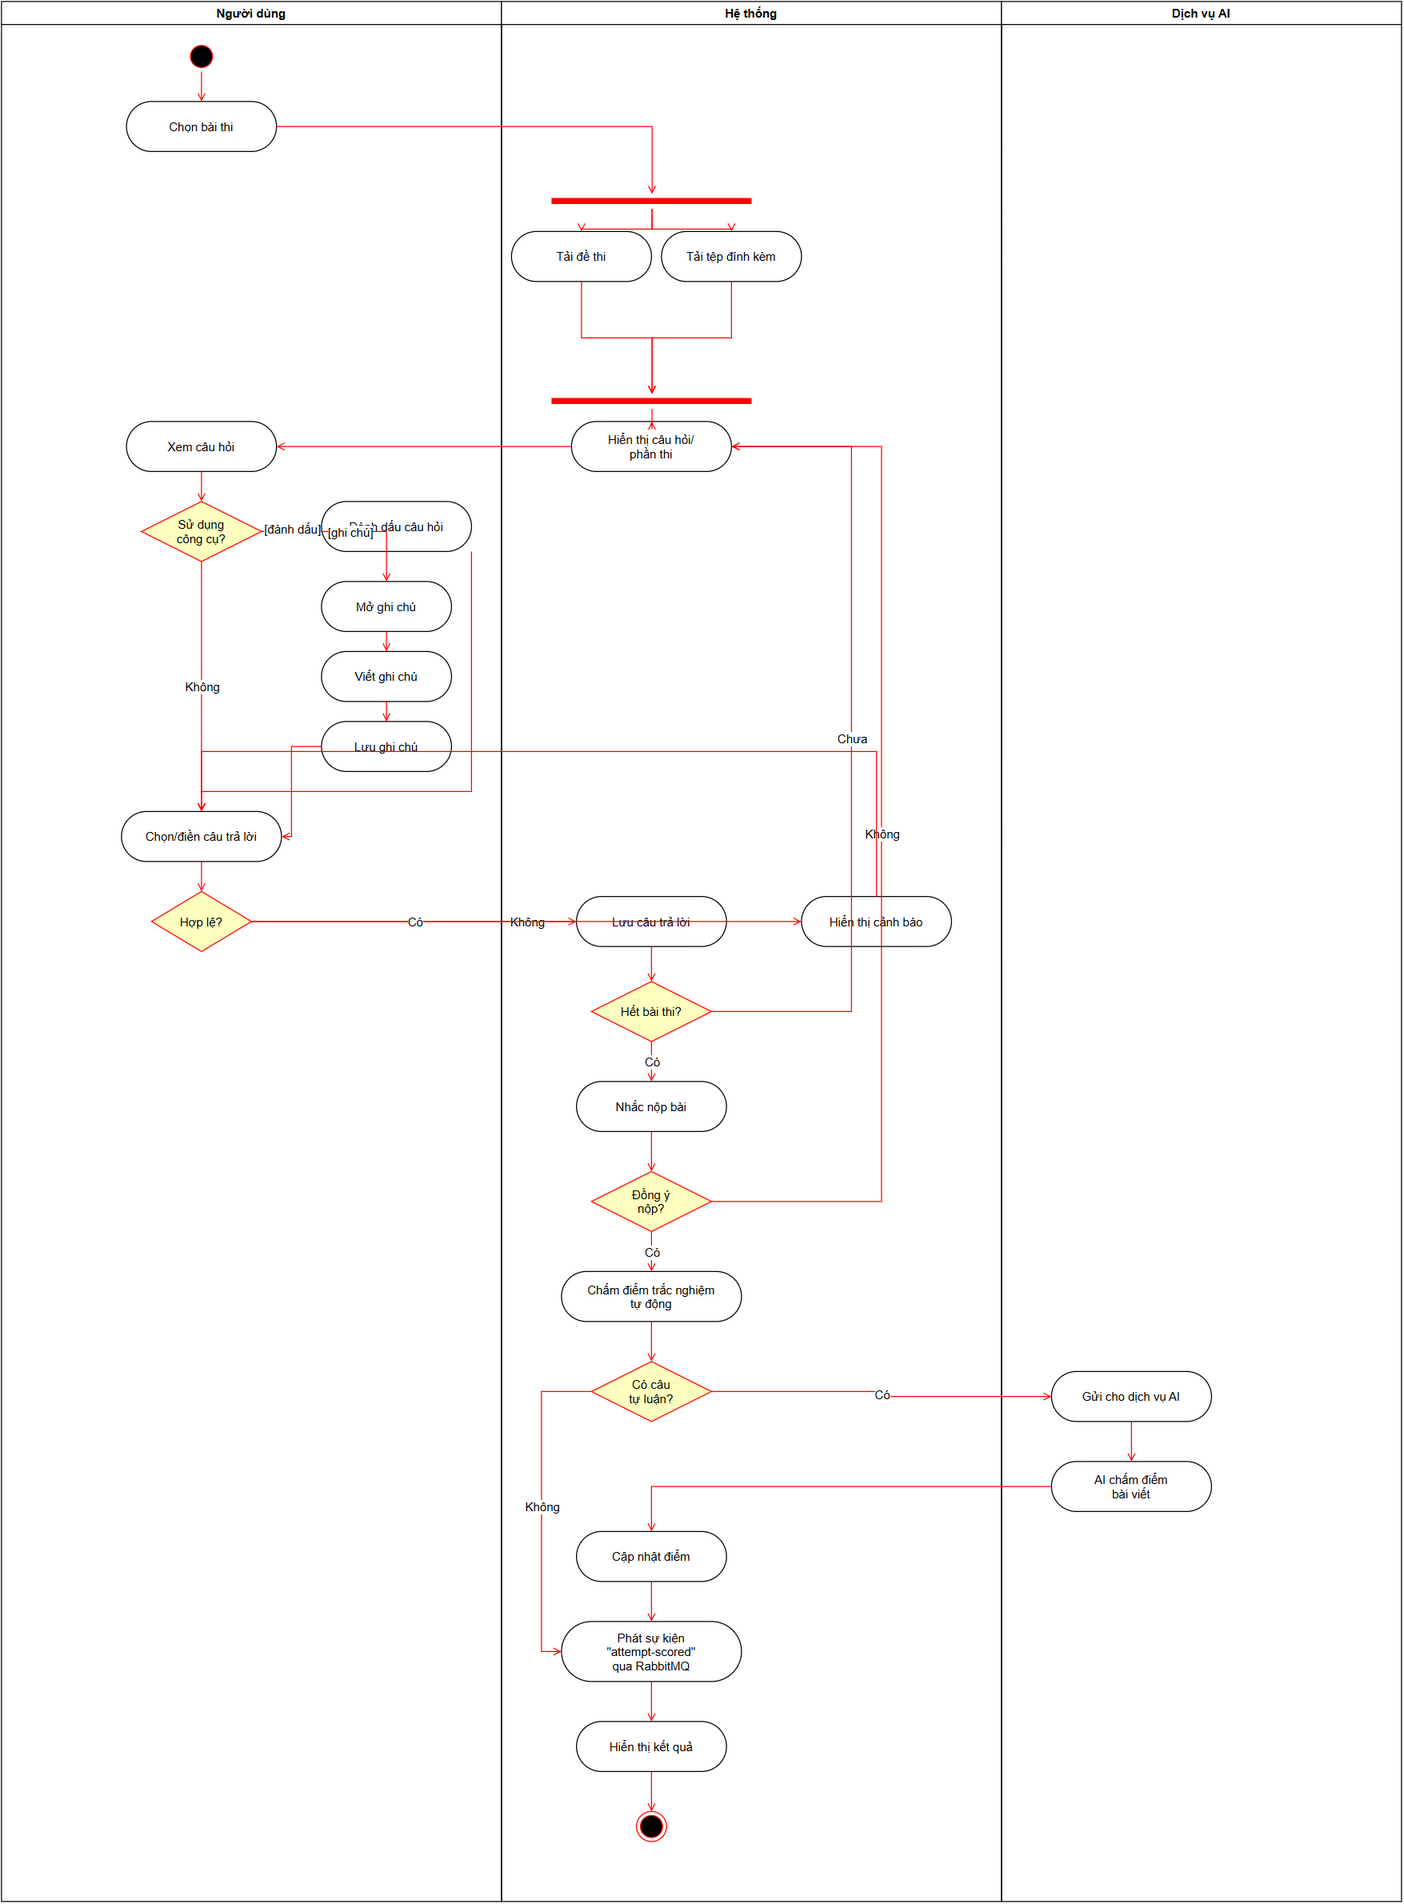
\includegraphics[width=\linewidth]{graphics/activity/lam_va_cham_diem_bai_thi}
        \captionsetup{skip=5pt}
        \caption{Activity diagram cho quy trình ``Làm và chấm điểm bài thi''}
        \label{ADLamThi}
\end{figure}

Hình~\ref{ADLamThi} minh họa luồng xử lý từ khi người dùng bắt đầu một attempt cho đến khi nhận kết quả. Quy trình bao gồm: chọn bài thi, trả lời từng câu hỏi (với khả năng đánh dấu và ghi chú), nộp bài, và chấm điểm tự động. Đối với câu hỏi dạng Writing, hệ thống kích hoạt pipeline chấm điểm AI bất đồng bộ thông qua RabbitMQ event bus.

\subsection{Quy trình tạo và quản lý đề thi}
\begin{figure}[H]
        \centering
        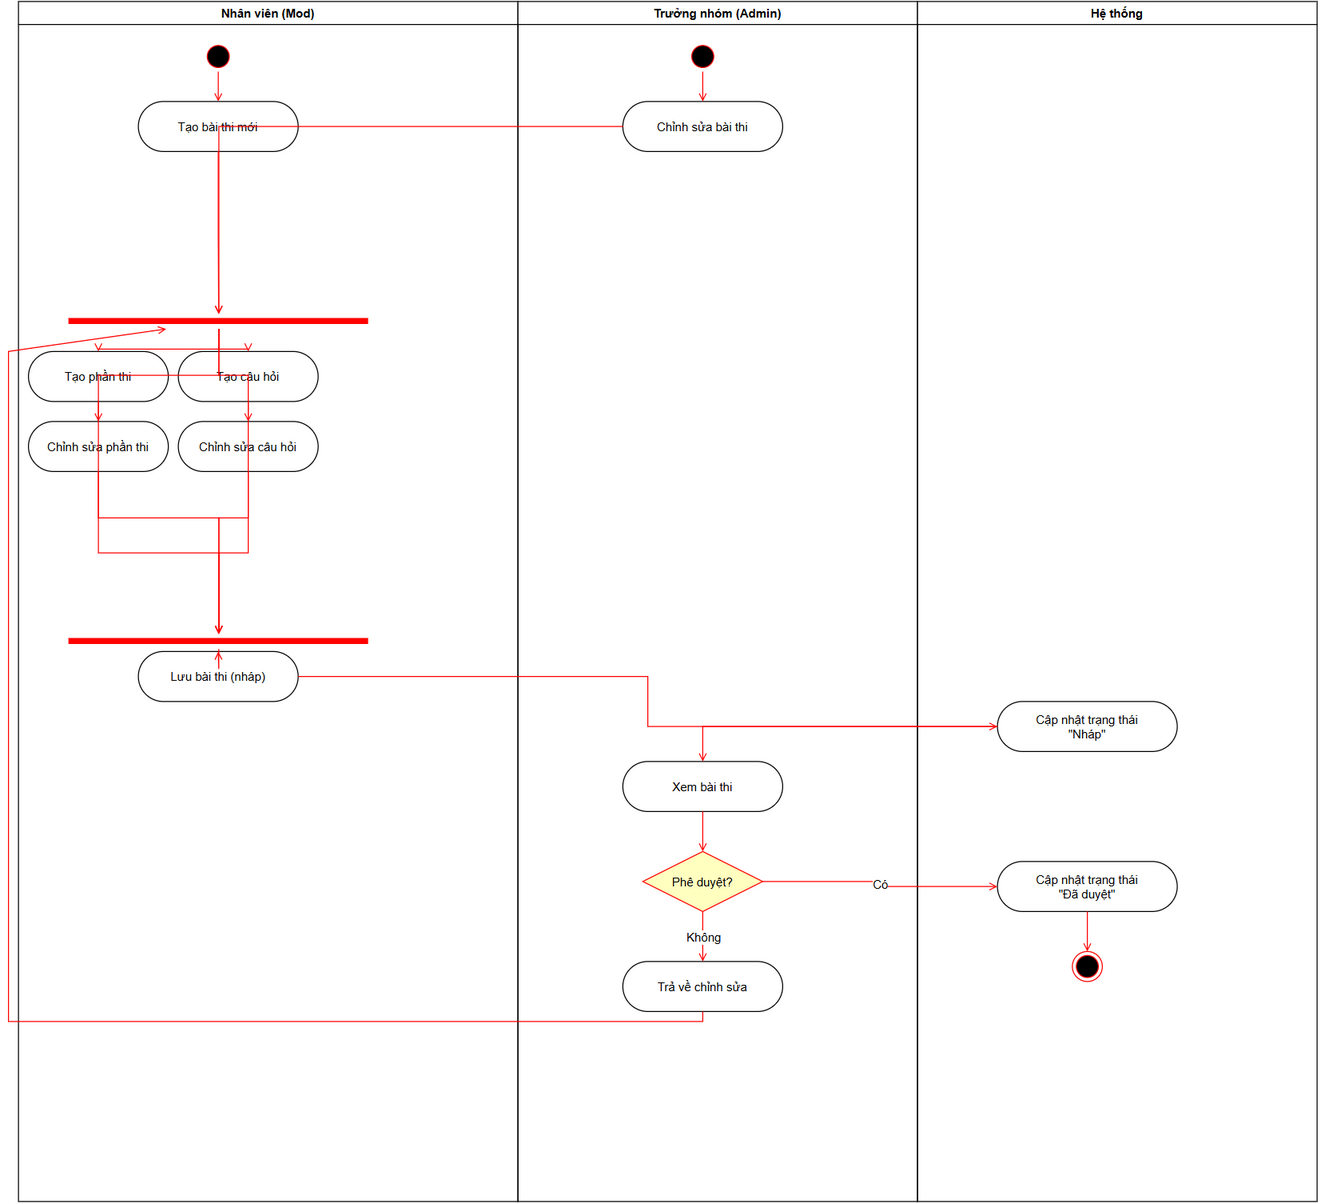
\includegraphics[width=\linewidth]{graphics/activity/tao_va_quan_ly_de_thi}
        \captionsetup{skip=5pt}
        \caption{Activity diagram cho quy trình ``Tạo và quản lý đề thi''}
        \label{ADQuanLyDeThi}
\end{figure}

Hình~\ref{ADQuanLyDeThi} mô tả quy trình phối hợp giữa Nhân viên (Mod) và Trưởng nhóm (Admin) trong việc soạn thảo đề thi. Nhân viên tạo exam, thêm section và question, sau đó lưu dưới dạng draft. Admin review và phê duyệt hoặc yêu cầu chỉnh sửa. Khi được phê duyệt, exam chuyển sang trạng thái published và hiển thị cho người học.

\subsection{Quy trình luyện nói AI}
\begin{figure}[H]
        \centering
        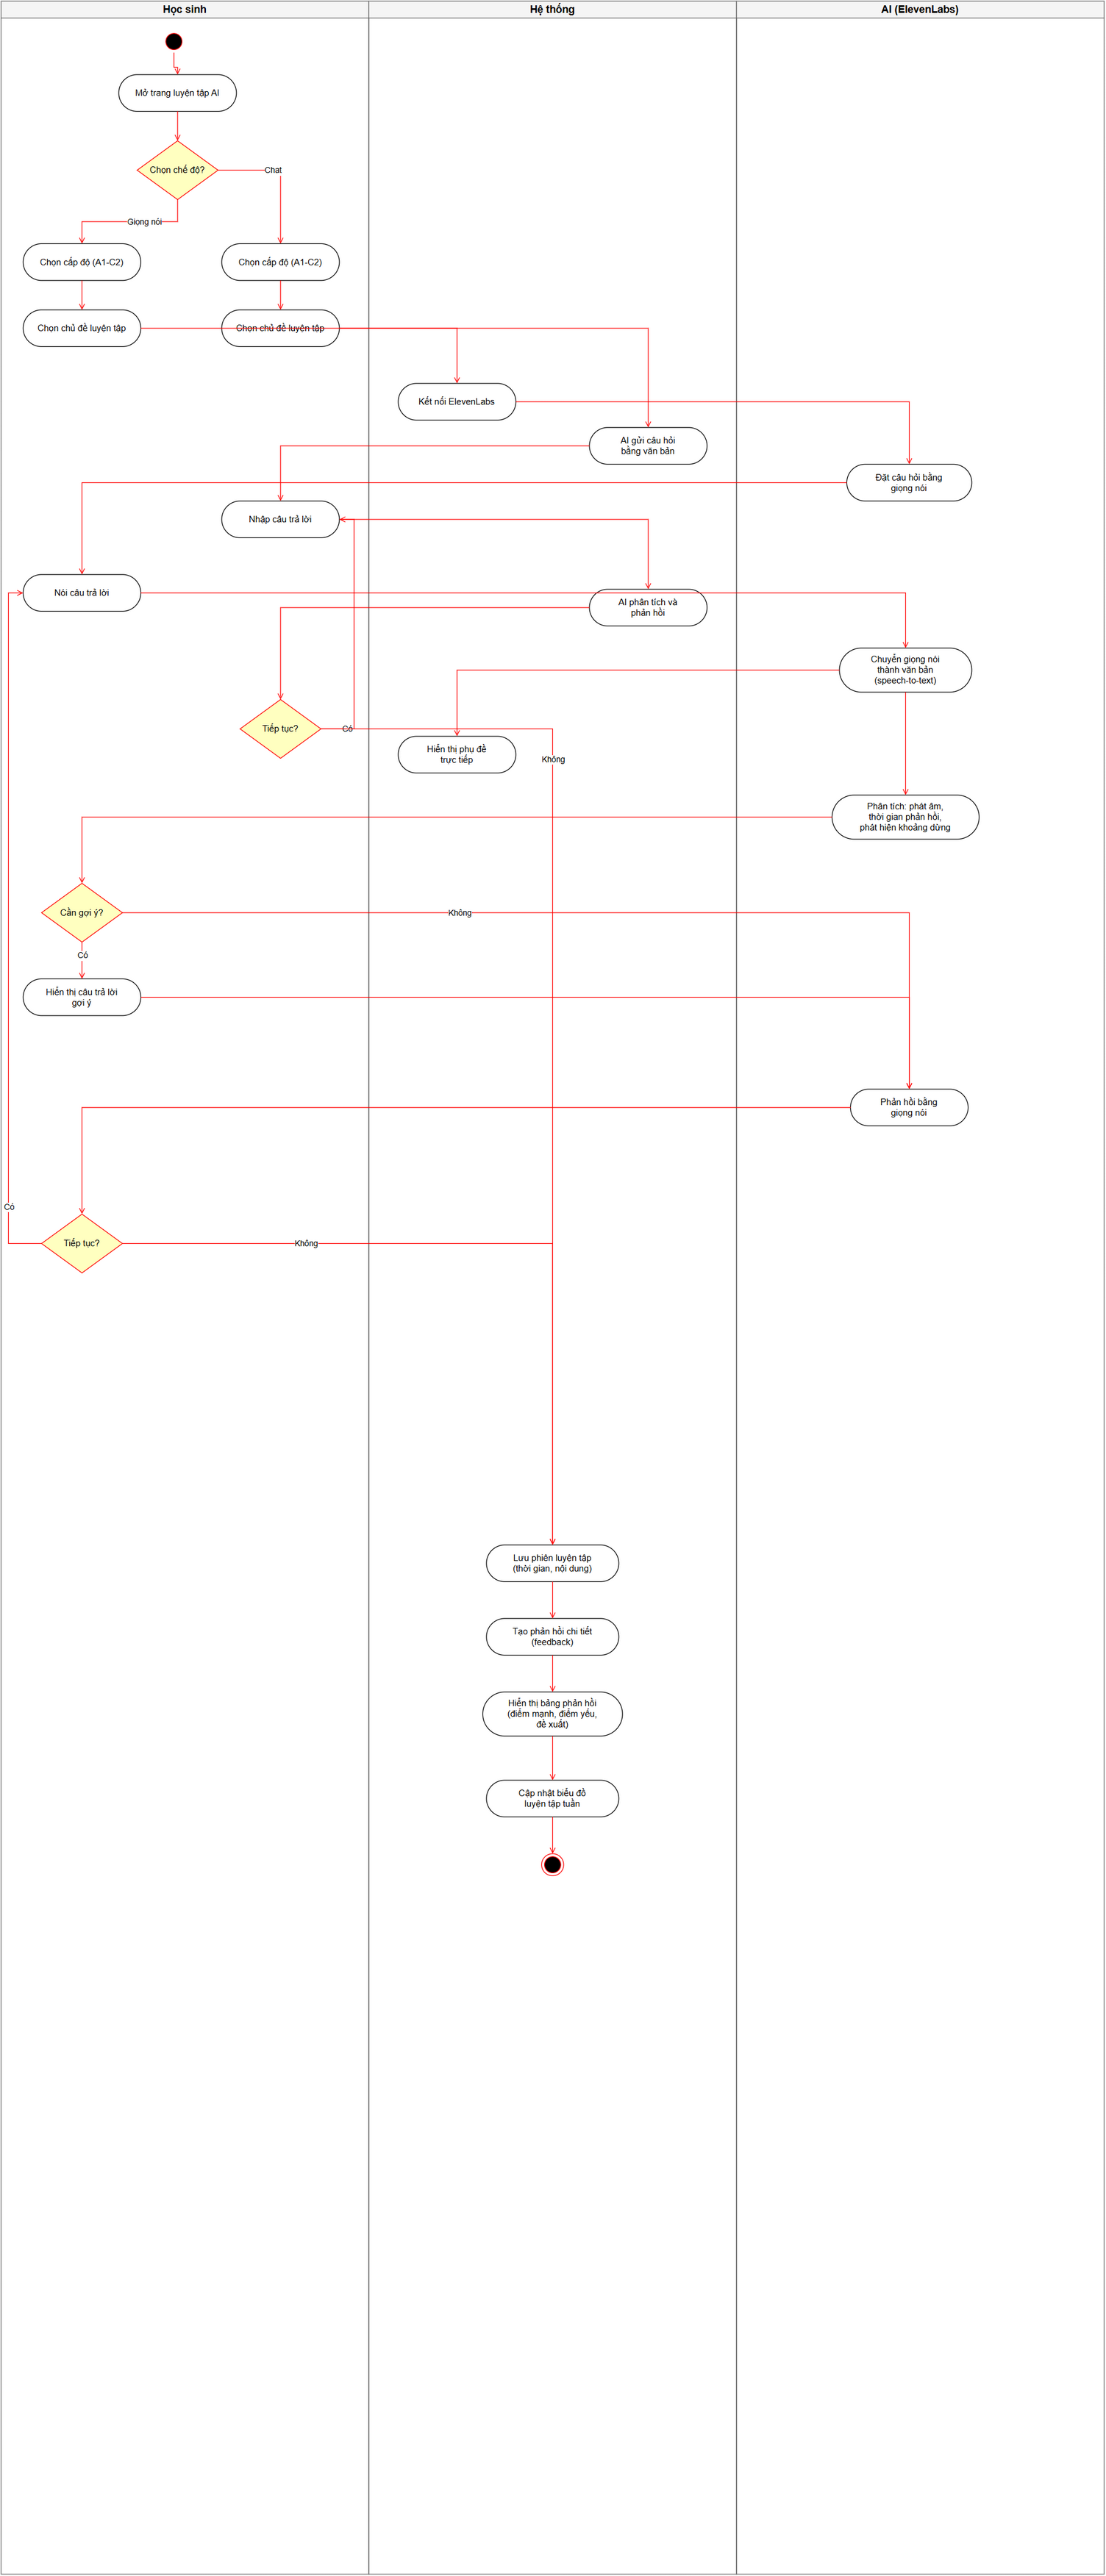
\includegraphics[width=\linewidth]{graphics/activity/luyen_noi_ai}
        \captionsetup{skip=5pt}
        \caption{Activity diagram cho quy trình ``Luyện nói với AI''}
        \label{ADLuyenNoiAI}
\end{figure}

Hình~\ref{ADLuyenNoiAI} minh họa luồng xử lý của phiên luyện nói AI sử dụng ElevenLabs. Học sinh chọn chủ đề và mức độ, sau đó tương tác hội thoại với AI tutor. Hệ thống thu thập dữ liệu phát âm, phân tích fluency, và cung cấp feedback chi tiết sau mỗi phiên.

\subsection{Quy trình học tập blended learning}
\begin{figure}[H]
        \centering
        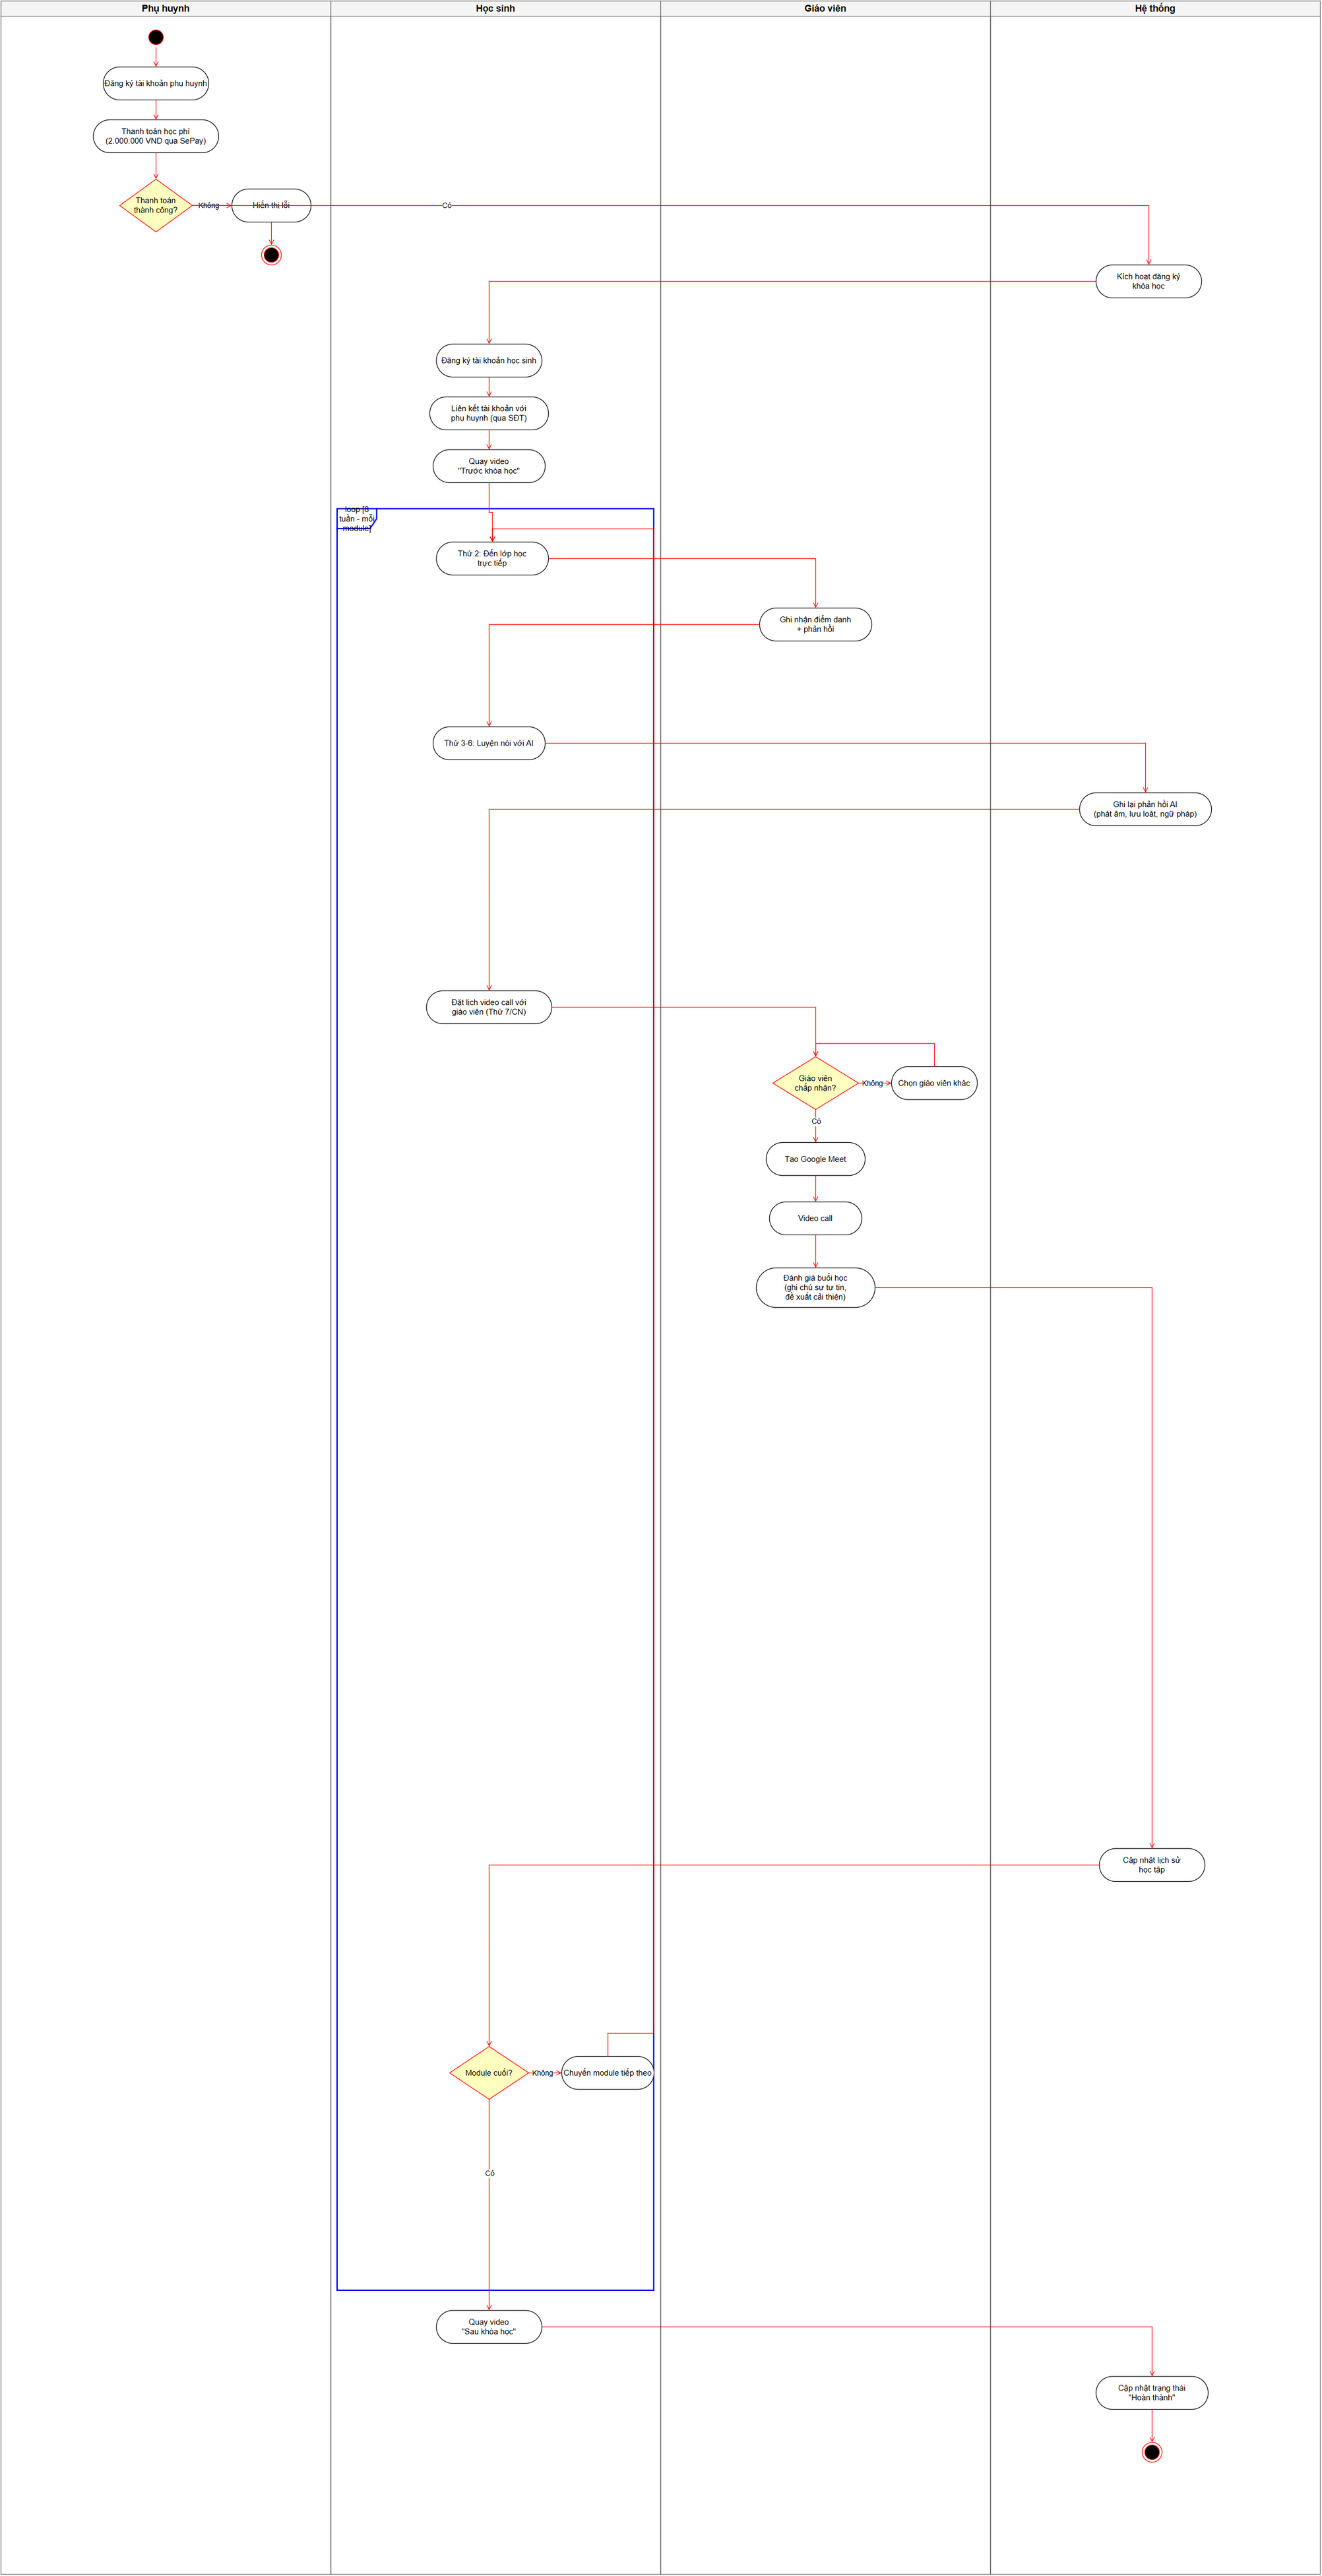
\includegraphics[width=\linewidth]{graphics/activity/qua_trinh_hoc_tap}
        \captionsetup{skip=5pt}
        \caption{Activity diagram cho quy trình ``Quá trình học tập hàng tuần''}
        \label{ADHocTap}
\end{figure}

Hình~\ref{ADHocTap} mô tả chu trình học tập hàng tuần theo mô hình blended learning: học trực tiếp vào thứ Hai, luyện nói AI từ thứ Ba đến thứ Sáu, và video call với giáo viên vào cuối tuần. Mỗi hoạt động được ghi nhận vào learning history với feedback tương ứng.

\subsection{Quy trình thanh toán}
\begin{figure}[H]
        \centering
        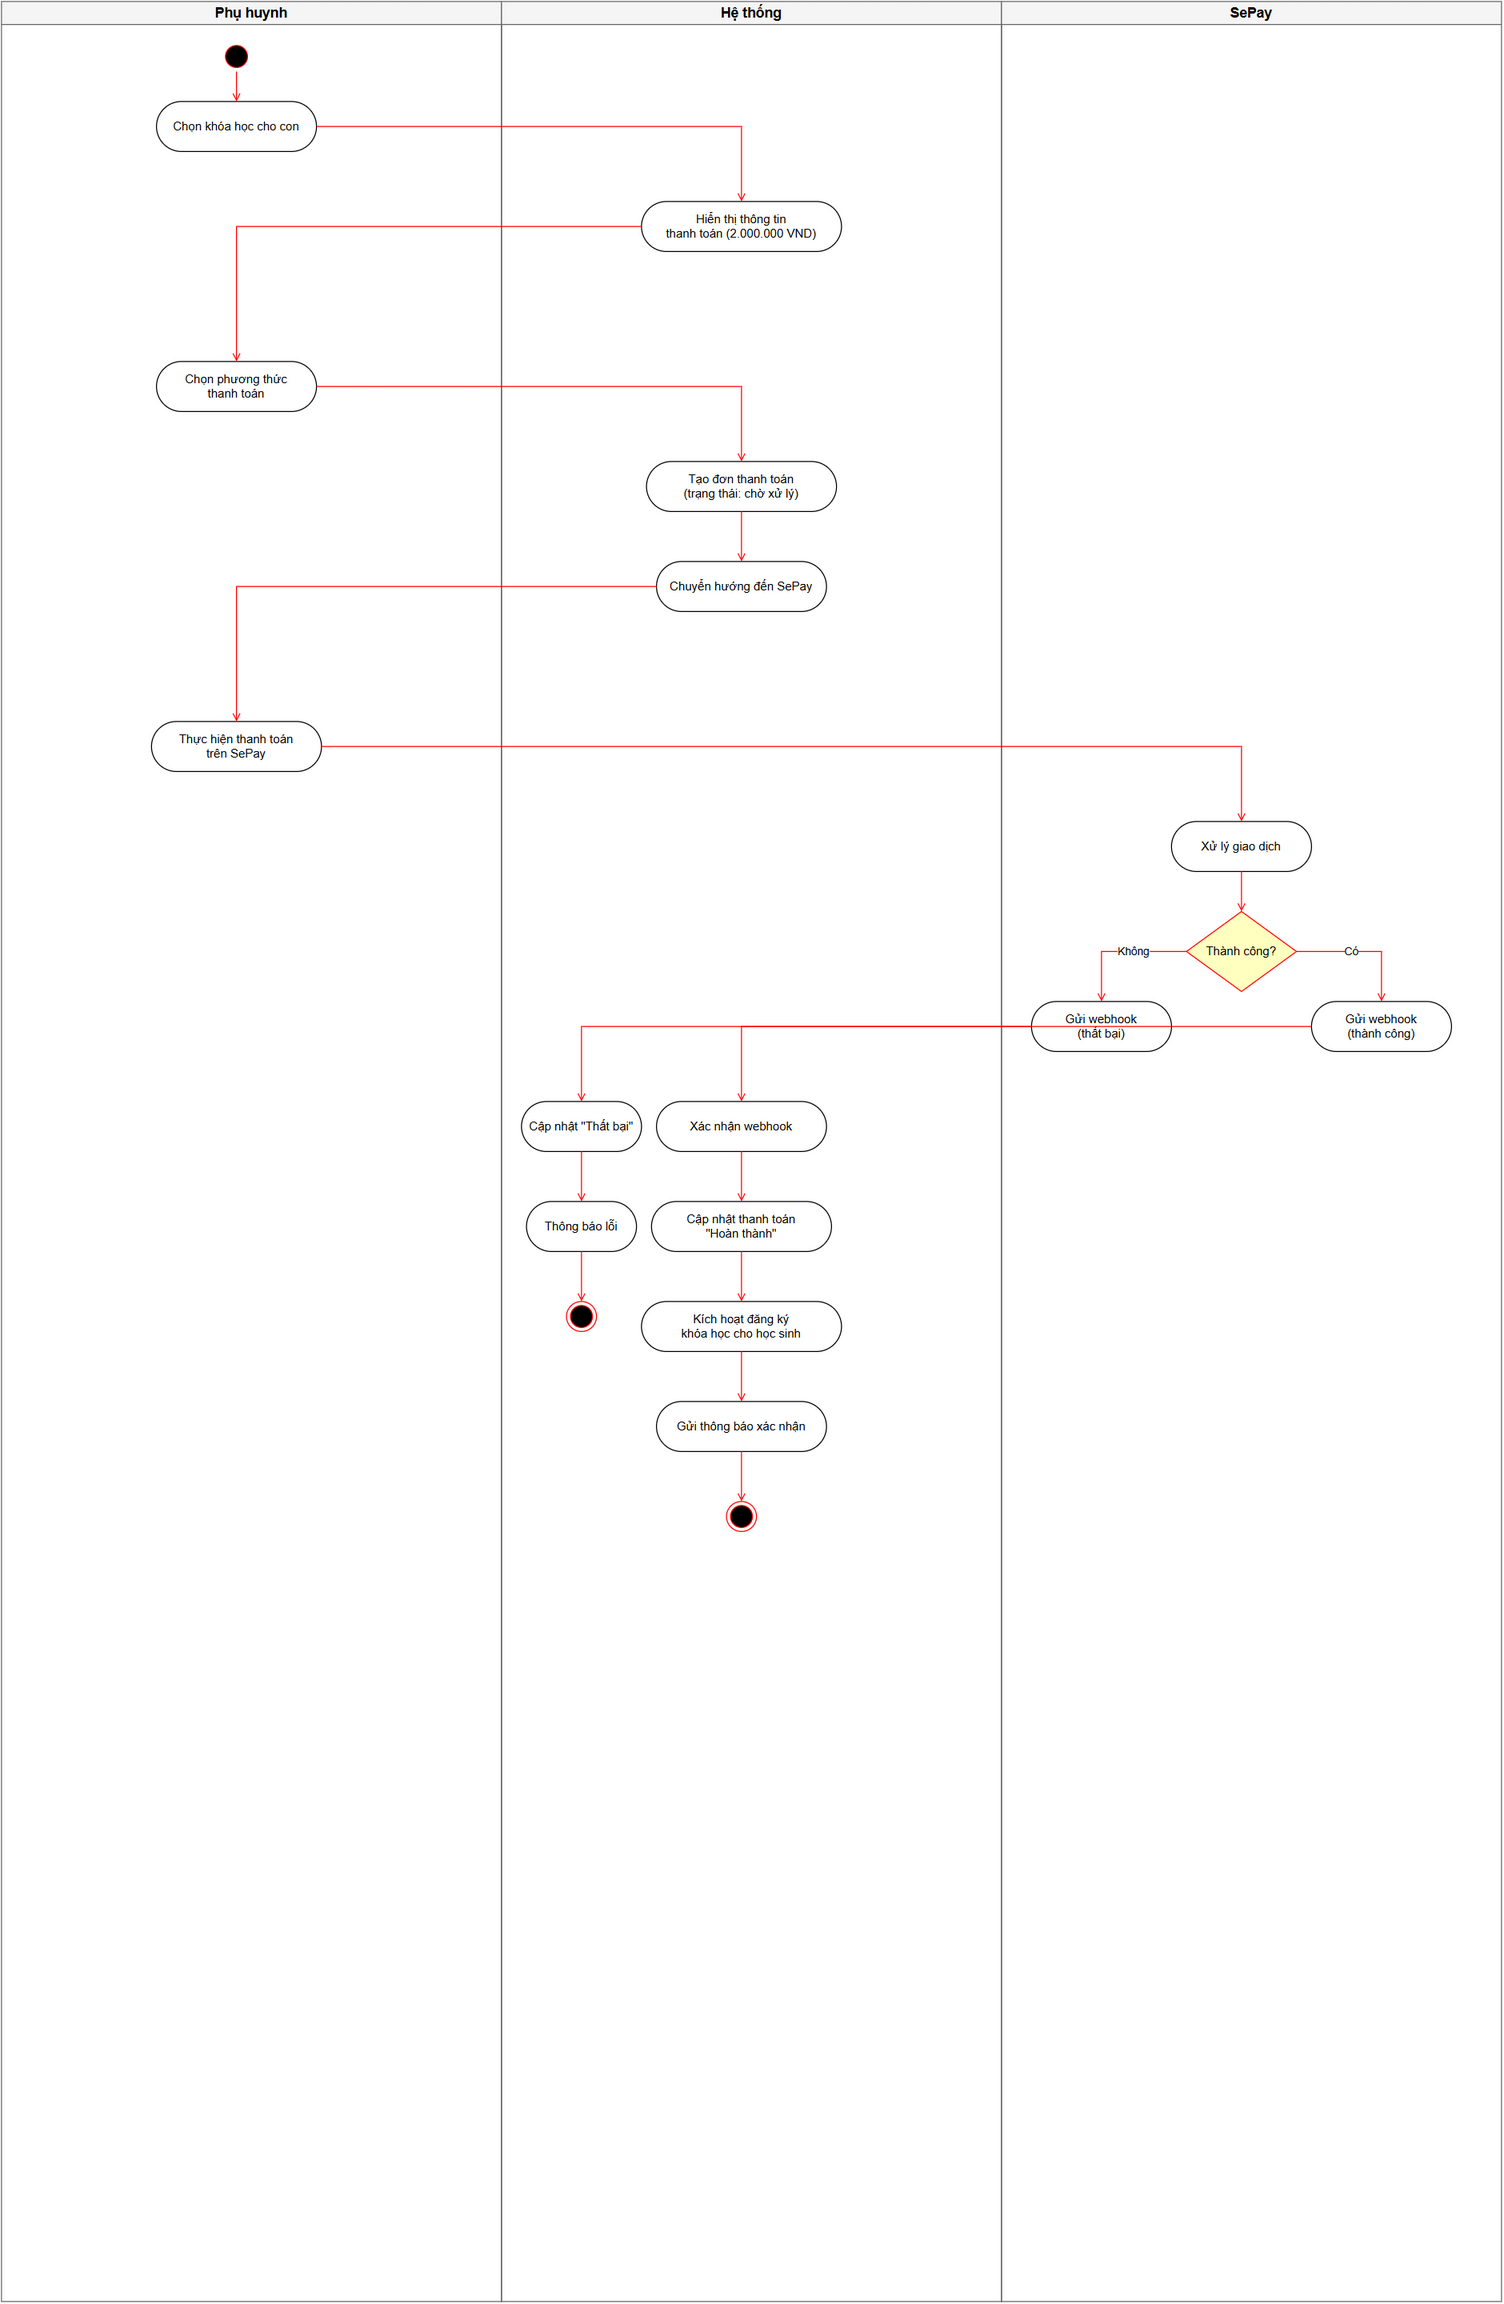
\includegraphics[width=\linewidth]{graphics/activity/thanh_toan}
        \captionsetup{skip=5pt}
        \caption{Activity diagram cho quy trình ``Thanh toán khóa học''}
        \label{ADThanhToan}
\end{figure}

Hình~\ref{ADThanhToan} minh họa luồng thanh toán qua cổng SePay. Phụ huynh khởi tạo thanh toán cho học sinh, hệ thống tạo payment record ở trạng thái pending, sau đó nhận webhook xác nhận từ SePay để cập nhật trạng thái enrollment.

\subsection{Quy trình hệ thống huy hiệu}
\begin{figure}[H]
        \centering
        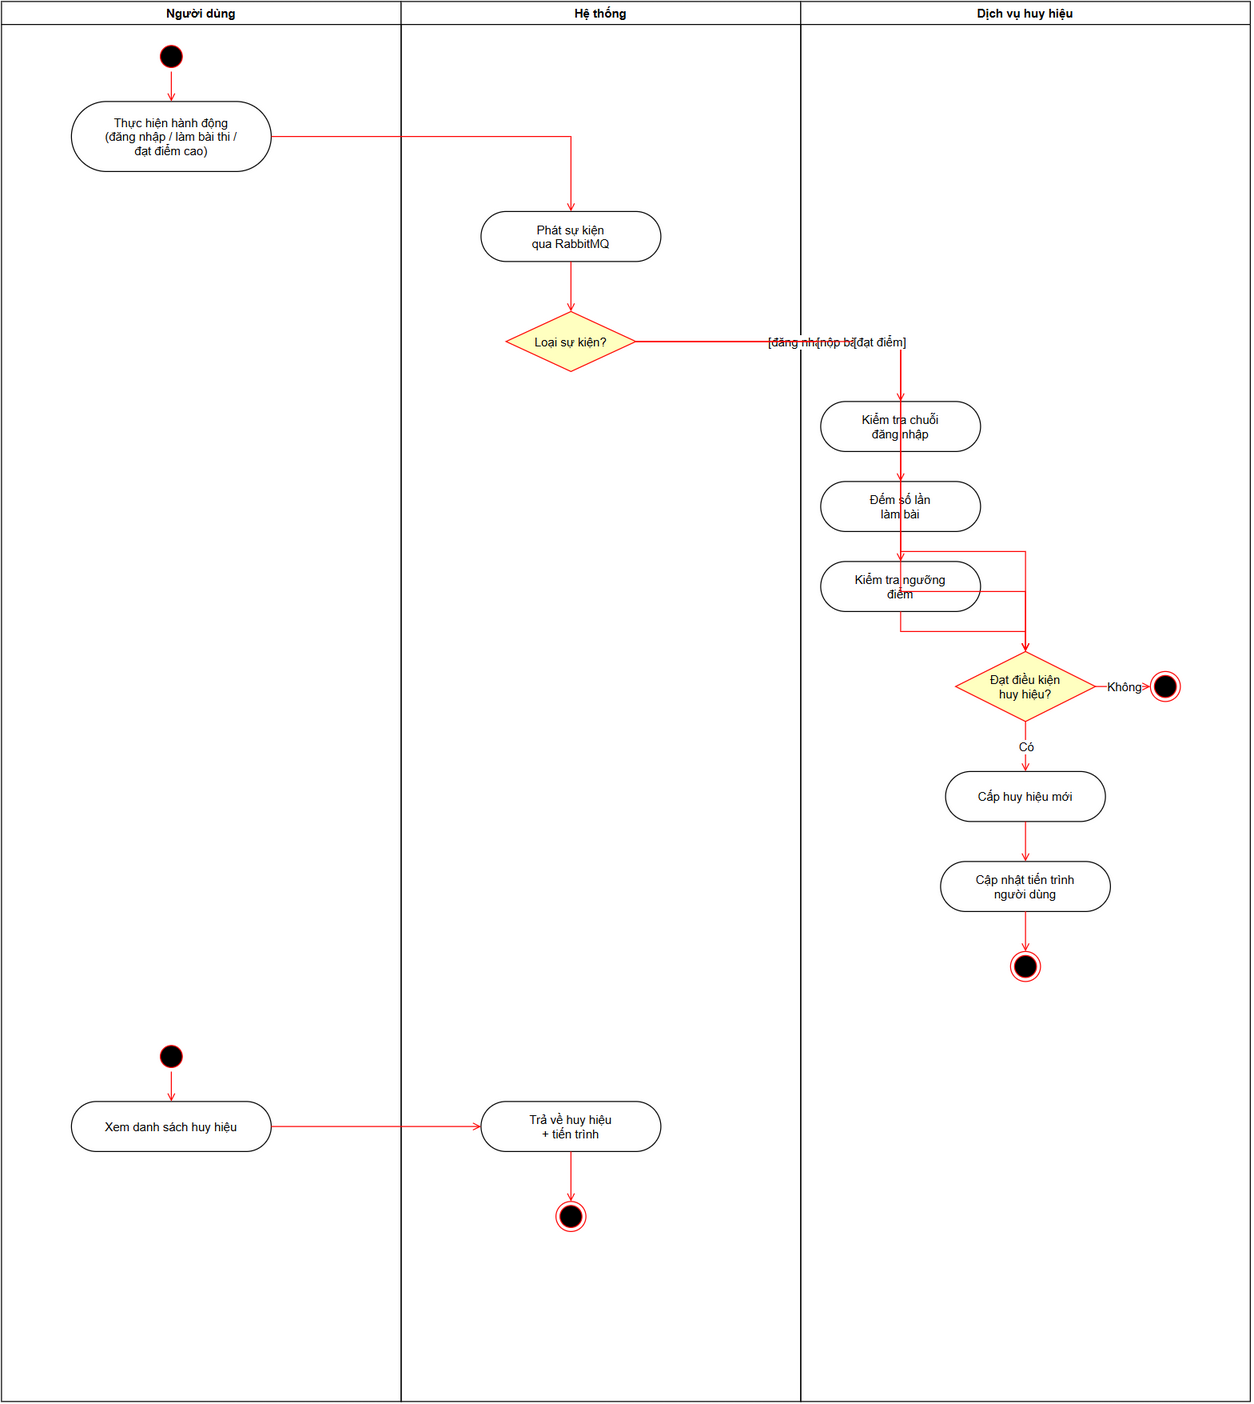
\includegraphics[width=\linewidth]{graphics/activity/he_thong_huy_hieu}
        \captionsetup{skip=5pt}
        \caption{Activity diagram cho quy trình ``Hệ thống huy hiệu và thành tích''}
        \label{ADHuyHieu}
\end{figure}

Hình~\ref{ADHuyHieu} mô tả cơ chế trao huy hiệu event-driven. Khi người dùng thực hiện các hành động (đăng nhập, nộp bài, đạt điểm cao), các event được publish qua RabbitMQ. Achievement service lắng nghe và đánh giá điều kiện nhận huy hiệu dựa trên các badge manager chuyên biệt.

\subsection{Quy trình thông báo}
\begin{figure}[H]
        \centering
        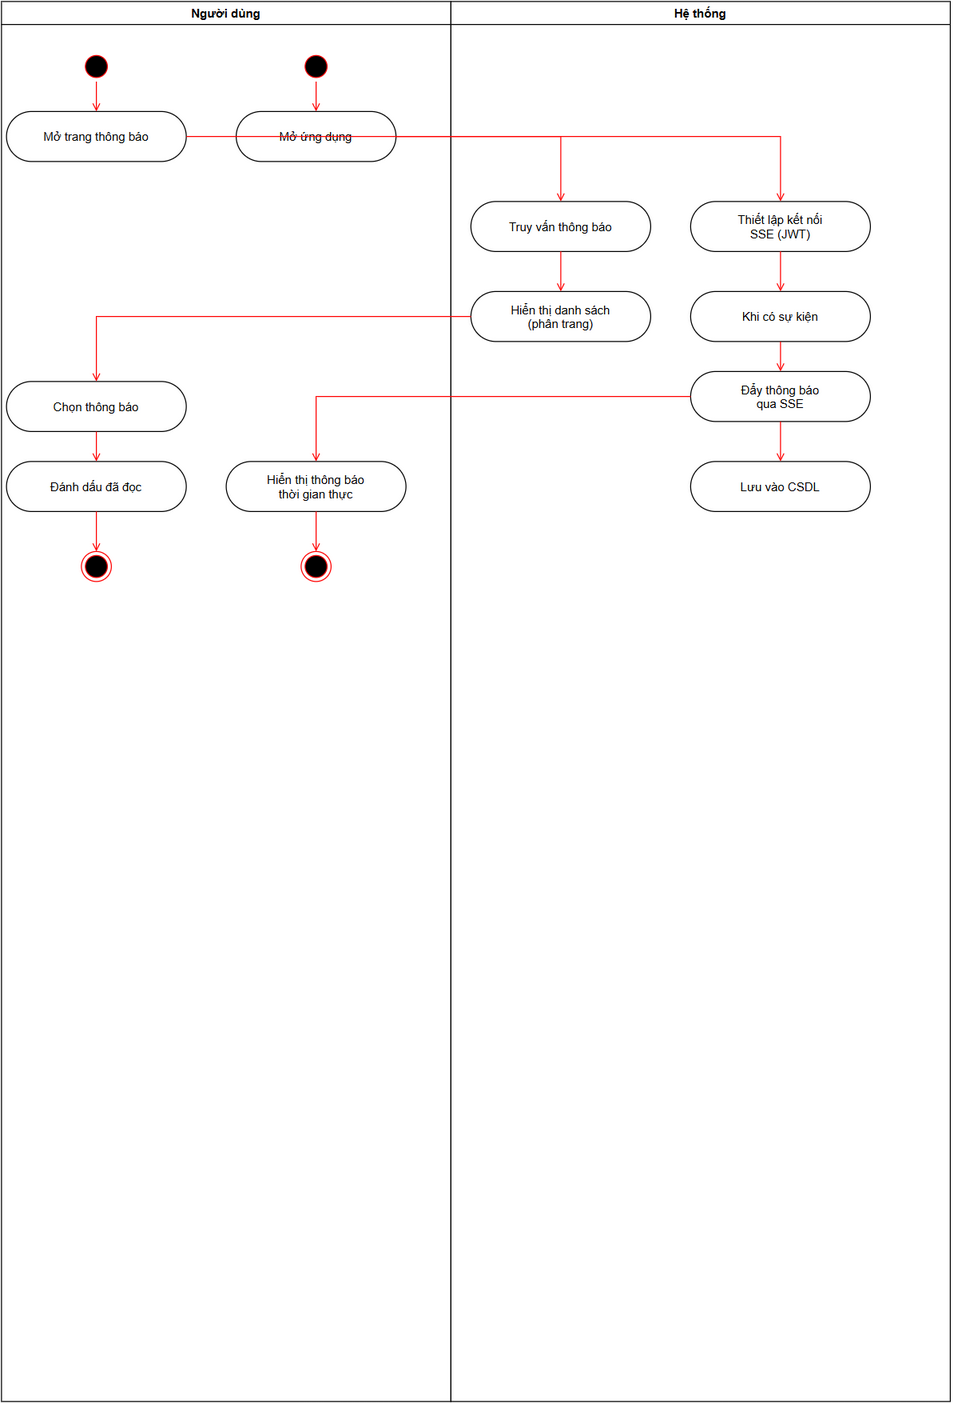
\includegraphics[width=\linewidth]{graphics/activity/thong_bao}
        \captionsetup{skip=5pt}
        \caption{Activity diagram cho quy trình ``Thông báo''}
        \label{ADThongBao}
\end{figure}

Hình~\ref{ADThongBao} minh họa luồng xử lý thông báo trong hệ thống, bao gồm các loại: yêu cầu kết nối tài khoản, xác nhận kết nối, nhắc nhở lịch booking, và thông báo chung.

%% ============================
\section{Biểu đồ tuần tự}

Phần này trình bày các biểu đồ tuần tự (Sequence Diagram), mô tả chi tiết luồng tương tác giữa các thành phần hệ thống theo trình tự thời gian cho từng quy trình nghiệp vụ.

\subsection{Làm và chấm điểm bài thi}
\begin{figure}[H]
        \centering
        
\includegraphics[width=\linewidth]{graphics/sequence/lam_va_cham_diem_bai_thi}
        \captionsetup{skip=5pt}
        \caption{Sequence diagram --- Làm và chấm điểm bài thi}
        \label{SDLamThi}
\end{figure}

Hình~\ref{SDLamThi} trình bày luồng tương tác giữa Client, Gateway, Exam Service và AI Scorer trong quá trình làm bài thi. Request đi qua Gateway (REST) tới Exam Service (gRPC), câu trả lời được lưu incrementally, và khi submit, event \texttt{attempt-submitted} được publish qua RabbitMQ để kích hoạt chấm điểm Writing bất đồng bộ.

\subsection{Tạo và quản lý đề thi}
\begin{figure}[H]
        \centering
        
\includegraphics[width=\linewidth]{graphics/sequence/tao_va_quan_ly_de_thi}
        \captionsetup{skip=5pt}
        \caption{Sequence diagram --- Tạo và quản lý đề thi}
        \label{SDQuanLyDeThi}
\end{figure}

Hình~\ref{SDQuanLyDeThi} mô tả luồng giao tiếp khi Mod/Admin tạo và quản lý đề thi. Các command (CreateExam, AddSection, AddQuestion) đi qua Gateway tới Exam Service, nơi áp dụng mẫu CQRS --- command handler xử lý ghi, query handler xử lý đọc.

\subsection{Luyện nói AI}
\begin{figure}[H]
        \centering
        
\includegraphics[width=\linewidth]{graphics/sequence/luyen_noi_ai}
        \captionsetup{skip=5pt}
        \caption{Sequence diagram --- Luyện nói với AI (ElevenLabs)}
        \label{SDLuyenNoiAI}
\end{figure}

Hình~\ref{SDLuyenNoiAI} minh họa luồng tương tác real-time giữa Client, Backend API và ElevenLabs trong phiên luyện nói. Audio được gửi tới ElevenLabs để speech-to-text, AI phản hồi giọng nói, và feedback được tổng hợp sau phiên.

\subsection{Quá trình học tập}
\begin{figure}[H]
        \centering
        
\includegraphics[width=\linewidth]{graphics/sequence/qua_trinh_hoc_tap}
        \captionsetup{skip=5pt}
        \caption{Sequence diagram --- Quá trình học tập hàng tuần}
        \label{SDHocTap}
\end{figure}

Hình~\ref{SDHocTap} trình bày luồng giao tiếp giữa các thành phần trong chu trình học tập hàng tuần, bao gồm việc ghi nhận hoạt động vào learning history và thu thập feedback từ AI, giáo viên, và lớp học trực tiếp.

\subsection{Thanh toán}
\begin{figure}[H]
        \centering
        
\includegraphics[width=\linewidth]{graphics/sequence/thanh_toan}
        \captionsetup{skip=5pt}
        \caption{Sequence diagram --- Thanh toán qua SePay}
        \label{SDThanhToan}
\end{figure}

Hình~\ref{SDThanhToan} mô tả luồng tương tác giữa Client, Backend, SePay Gateway và Database trong quy trình thanh toán. Backend tạo payment record, SePay gửi webhook xác nhận, và enrollment status được cập nhật tương ứng.

\subsection{Hệ thống huy hiệu}
\begin{figure}[H]
        \centering
        
\includegraphics[width=\linewidth]{graphics/sequence/he_thong_huy_hieu}
        \captionsetup{skip=5pt}
        \caption{Sequence diagram --- Hệ thống huy hiệu event-driven}
        \label{SDHuyHieu}
\end{figure}

Hình~\ref{SDHuyHieu} minh họa kiến trúc event-driven của hệ thống huy hiệu. Các service (Auth, Exam) publish event qua RabbitMQ, Achievement Service consume và đánh giá điều kiện badge thông qua các manager chuyên biệt (LoginBadgeManager, AttemptCounterBadgeManager, AttemptScoreBadgeManager).

\subsection{Thông báo}
\begin{figure}[H]
        \centering
        
\includegraphics[width=\linewidth]{graphics/sequence/thong_bao}
        \captionsetup{skip=5pt}
        \caption{Sequence diagram --- Luồng thông báo}
        \label{SDThongBao}
\end{figure}

Hình~\ref{SDThongBao} trình bày luồng tạo và phân phối thông báo. Khi các sự kiện xảy ra (kết nối tài khoản, đặt lịch), notification record được tạo trong database và có thể được push tới client qua REST API hoặc SSE.

%% ============================
\section{Thiết kế kiến trúc}
\subsection{Đặc trưng kiến trúc}
Từ quá trình phân tích các yêu cầu phi chức năng, chúng tôi có thể xác định các đặc trưng sau của kiến trúc hệ thống:
\begin{itemize}
  \item Performance
  \item Scalability
  \item Availability
  \item Portability
  \item Security
  \item Maintainability
\end{itemize}

Từ các đặc trưng đã được rút ra, chúng tôi xác định các đặc trưng then chốt. Có ba đặc trưng chính cần được ưu tiên như sau:


{\scriptsize
\setlength{\tabcolsep}{4pt}
\renewcommand{\arraystretch}{1.5}
\begin{tabularx}{\textwidth}{|>{\centering\arraybackslash}m{3cm}|>{\arraybackslash}X|}
\hline
\textbf{NFR Name} & \textbf{Mô tả} \\ \hline
Scalability & Hệ thống phải hỗ trợ việc bổ sung tính năng mới hoặc xử lý khối lượng lớn người dùng mà không cần thay đổi căn bản kiến trúc (NF-2). Điều này bảo đảm khả năng mở rộng mượt mà khi nhu cầu tăng lên. \\ \hline
High Availability & Hệ thống phải vận hành liên tục với mức 99.9\% uptime (NF-3), bảo đảm người dùng có thể truy cập không gián đoạn. High availability là yếu tố quan trọng để duy trì niềm tin của người dùng và reliability của dịch vụ. \\ \hline
Security & Hệ thống phải bảo vệ sensitive data và tuân thủ các security standard (NF-5), bảo đảm chỉ những người dùng được authorized mới có thể truy cập thông tin quan trọng. \\ \hline
\caption{Các đặc trưng then chốt}
\end{tabularx}}


Bên cạnh các đặc trưng chính, một số thuộc tính bổ sung cũng cần được xem xét để bảo đảm tính ổn định và maintainability trong dài hạn:


{\scriptsize
\setlength{\tabcolsep}{4pt}
\renewcommand{\arraystretch}{1.5}
\begin{tabularx}{\textwidth}{|>{\centering\arraybackslash}m{4cm}|>{\arraybackslash}X|}
\hline
\textbf{NFR Name} & \textbf{Mô tả} \\ \hline
Performance & Bảo đảm thời gian phản hồi nhanh cho trang, các tác vụ AI evaluation và API operation (NF-1). \\ \hline
Modular Independence & Các module có thể được phát triển, kiểm thử và thay thế một cách độc lập (NF-2), từ đó cải thiện maintainability và giảm rủi ro phát sinh side effect ngoài ý muốn. \\ \hline
Portability and Maintainability & Hệ thống cần dễ bảo trì và có tính portable giữa các môi trường (NF-4, NF-6), cho phép deployment và update diễn ra thuận lợi. \\ \hline
Elasticity & Hệ thống cần xử lý được các đợt tăng traffic đột biến mà không làm suy giảm performance (NF-2). \\ \hline
Legality \& Compliance & Hệ thống phải tuân thủ các yêu cầu pháp lý và quy định liên quan, đặc biệt về data security và user privacy (NF-5). \\ \hline
\caption{Các đặc trưng hàm ẩn cho tính ổn định dài hạn}
\end{tabularx}}


\subsection{So sánh các kiến trúc}
\subsection{Kiến trúc Layered}
Kiến trúc Layered được tổ chức thành nhiều layer, mỗi layer đảm nhận một trách nhiệm cụ thể. Mặc dù kiến trúc này cung cấp separation of concerns rõ ràng, khả năng Scalability của nó bị giới hạn do sự tight coupling giữa các layer. High availability cũng khó đạt được vì mọi layer phụ thuộc lẫn nhau. Security có thể được quản lý ở từng layer, nhưng việc thực thi đồng nhất trên toàn hệ thống lại không đơn giản. Recovery khá phức tạp vì lỗi ở một layer có thể ảnh hưởng đến toàn bộ hệ thống. Tính độc lập giữa các module thấp, và maintainability có thể trở nên cồng kềnh khi hệ thống phát triển lớn hơn. Việc integration với các hệ thống bên ngoài là khả thi nhưng kém linh hoạt hơn so với các kiến trúc khác.

\subsubsection{Kiến trúc Modular Monolith}
Kiến trúc Modular Monolith cải thiện Scalability và Maintainability so với monolith thuần túy nhờ sự tách biệt giữa các module. Các module có thể được phát triển và chỉnh sửa tương đối độc lập, mặc dù High availability vẫn có thể khó bảo đảm vì các module còn phụ thuộc lẫn nhau. Security có thể được áp dụng ở cấp module, nhưng một lỗ hổng trong một module vẫn có thể ảnh hưởng đến toàn hệ thống. Recovery ở mức trung bình, do lỗi trong một module có thể tác động đến hệ thống. Khả năng integration bên trong hệ thống khá tốt, dù việc integration với các hệ thống bên ngoài vẫn kém linh hoạt hơn so với microservices hoặc các hướng tiếp cận event-driven.

\subsubsection{Kiến trúc Microkernel}
Kiến trúc Microkernel tách core system ra khỏi các plug-in module. Cách tiếp cận này cho phép mở rộng core functionality một cách dễ dàng và hỗ trợ các plugin hoạt động độc lập. High availability có thể đạt được tốt cho core system nhưng khó hơn đối với các plugin. Security mạnh ở phần lõi, tuy nhiên đòi hỏi phải cô lập plugin cẩn thận. Recovery đối với phần lõi khá trực tiếp, nhưng việc khôi phục plugin có thể khó hơn. Tính độc lập giữa các module và maintainability đều cao, đồng thời integration thông qua plugin khá tốt, dù việc kết nối với các hệ thống bên ngoài vẫn có thể gặp thách thức.

\subsubsection{Kiến trúc Microservices}
Kiến trúc Microservices mang lại Scalability cao, vì mỗi service có thể được phát triển, deployment và scale một cách độc lập. High availability cũng dễ đạt được hơn do các service có thể được triển khai trên nhiều instance. Security có thể được áp dụng riêng cho từng service, mặc dù việc quản lý security trên toàn bộ các service có thể khá phức tạp. Recovery rất mạnh vì lỗi ở một service không làm toàn bộ hệ thống dừng hoạt động. Tính độc lập của module và maintainability đều cao, dù độ phức tạp tổng thể của hệ thống tăng lên do cơ chế giao tiếp giữa các service. Integration được thực hiện tương đối trực tiếp thông qua APIs.

\subsubsection{Kết luận về kiến trúc}

{\scriptsize
\setlength{\tabcolsep}{4pt}
\renewcommand{\arraystretch}{1.5}
\begin{tabularx}{\textwidth}{|>{\centering\arraybackslash}m{4cm}|>{\centering\arraybackslash}m{2cm}|>{\centering\arraybackslash}m{2cm}|>{\centering\arraybackslash}m{2.5cm}|>{\centering\arraybackslash}m{2cm}|}
\hline
\textbf{Characteristic} & \textbf{Mono} & \textbf{Layered} & \textbf{Microservices} & \textbf{Microkernel} \\ \hline
Performance & 3 & 3 & 5 & 4 \\ \hline
Scalability & 2 & 3 & 5 & 3 \\ \hline
Availability & 2 & 3 & 5 & 3 \\ \hline
Portability & 3 & 3 & 5 & 4 \\ \hline
Security & 4 & 4 & 3 & 4 \\ \hline
Maintainability & 2 & 4 & 5 & 5 \\ \hline
\caption{So sánh các kiến trúc phần mềm theo các đặc trưng (1 = thấp, 5 = cao)}
\end{tabularx}
}


Dựa trên việc so sánh các kiến trúc theo những đặc trưng then chốt, có thể thấy rằng Microservices nhìn chung đạt điểm tổng thể cao nhất, đặc biệt nổi trội ở performance, scalability, availability, portability và maintainability. Microkernel cũng cho kết quả tốt, nhất là ở maintainability, security và performance, dù scalability và availability của nó thấp hơn đôi chút do phụ thuộc vào core system. Trong khi đó, các kiến trúc Layered và Mono bộc lộ nhiều hạn chế, đặc biệt ở scalability, availability và maintainability, do sự tight coupling và mức độ linh hoạt theo module thấp hơn. Vì vậy, đối với các hệ thống đòi hỏi khả năng phản hồi cao, tính modularity và khả năng scale độc lập cho từng thành phần, Microservices là kiến trúc phù hợp nhất; còn Microkernel có thể được cân nhắc cho các hệ thống ưu tiên tính linh hoạt của plugin và maintainability. Chúng tôi quyết định lựa chọn kiến trúc Microservices \cite{microservices_newman}.

\subsection{Tổng quan kiến trúc}
Để hỗ trợ phong cách kiến trúc Microservice, chúng tôi quyết định sử dụng mẫu kiến trúc ``Clean architecture'' \cite{clean_architecture} và áp dụng Domain Driven Design \cite{ddd_evans} theo hướng mềm dẻo (tức là dùng Domain-Driven Design như một định hướng linh hoạt thay vì bắt buộc tuân thủ cứng nhắc mọi mẫu thiết kế) trong mã nguồn.

Clean architecture là một cách tiếp cận thiết kế phần mềm nhấn mạnh sự tách biệt trách nhiệm và tính độc lập giữa framework, giao diện người dùng, cơ sở dữ liệu và các tác nhân bên ngoài. Ý tưởng chính là tổ chức mã nguồn theo các lớp, trong đó các entity ở lõi biểu diễn luật nghiệp vụ, bao quanh bởi các use case hiện thực logic đặc thù của ứng dụng, còn các lớp ngoài cùng xử lý giao diện, framework và hạ tầng. Các phụ thuộc luôn hướng vào trong, vì vậy logic lõi không bị ảnh hưởng khi hệ thống bên ngoài thay đổi. Điều này giúp hệ thống dễ bảo trì, dễ kiểm thử và dễ thích nghi với các thay đổi trong tương lai.

\begin{figure}[H]
        \centering
        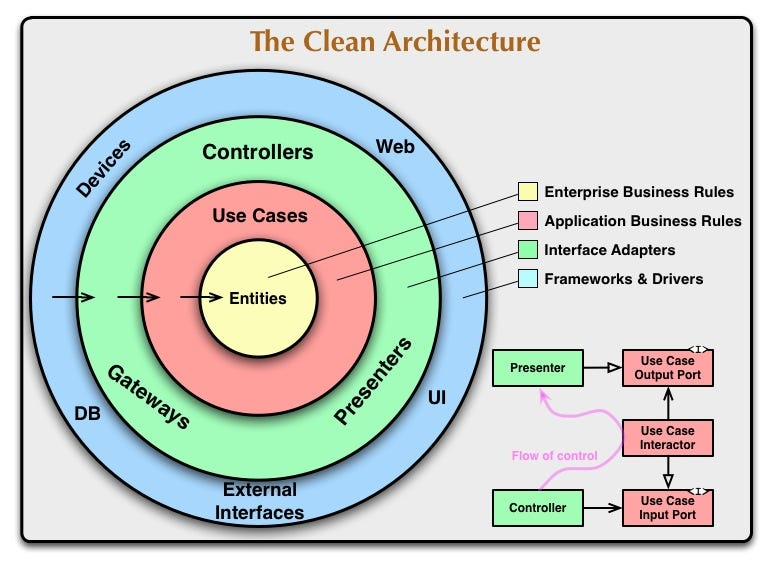
\includegraphics[width=0.75\linewidth]{graphics/architecture/clean}
        \captionsetup{skip=5pt}
        \caption{Tổng quan về mẫu Clean architecture}
\end{figure}

Tiếp theo, các microservice của chúng tôi bao gồm các thành phần chính sau:
\begin{itemize}
  \item API Gateway: Được sử dụng cho routing và tổng hợp dữ liệu. Thành phần này cũng có thể đóng vai trò là API Orchestrator, giúp điều phối và quản lý các lời gọi tới nhiều microservices, đồng thời trả về kết quả tổng hợp cho người dùng, từ đó giảm tải cho client và cải thiện performance của hệ thống.
  \item Auth Service: Được sử dụng để authenticate và authorize các request đi vào hệ thống. Những request ban đầu chưa được authenticated sẽ được API Gateway chuyển đến service này, sau đó được điều hướng tới login/register API. Các request tiếp theo sẽ đi qua service này để thực hiện authentication.
  \item Message Broker: Đóng vai trò trung gian trong việc truyền tải message giữa các service \cite{rabbitmq_docs}.
  \item AI Grade Service: Chịu trách nhiệm chấm điểm các bài làm Speaking/Writing.
  \item Blog Service: Một CRUD service dùng để quản lý blog.
  \item Exam Service: Chịu trách nhiệm xử lý mọi nghiệp vụ liên quan đến exam, bao gồm exam management cho nhân viên, exam attempt và history,...
  \item Flashcard Service: Một CRUD service dùng để quản lý flashcard.
  \item File Service: Chịu trách nhiệm quản lý và tối ưu việc truyền tải cũng như lưu trữ file.
\end{itemize}

\begin{figure}[H]
        \centering
        
\includegraphics[width=\linewidth]{graphics/architecture/Architecture}
        \captionsetup{skip=5pt}
        \caption{Tổng quan kiến trúc hệ thống}
       
\end{figure}

\section{Thiết kế cơ sở dữ liệu}

Do hệ thống áp dụng kiến trúc microservices \cite{microservices_newman}, mỗi service sở hữu cơ sở dữ liệu riêng biệt (database-per-service pattern). Phần này trình bày ERD cho từng service, phản ánh đúng schema vật lý đang được sử dụng trong mã nguồn (Prisma ORM \cite{prisma_docs}).

\subsection{Auth Service}
\begin{figure}[H]
        \centering
        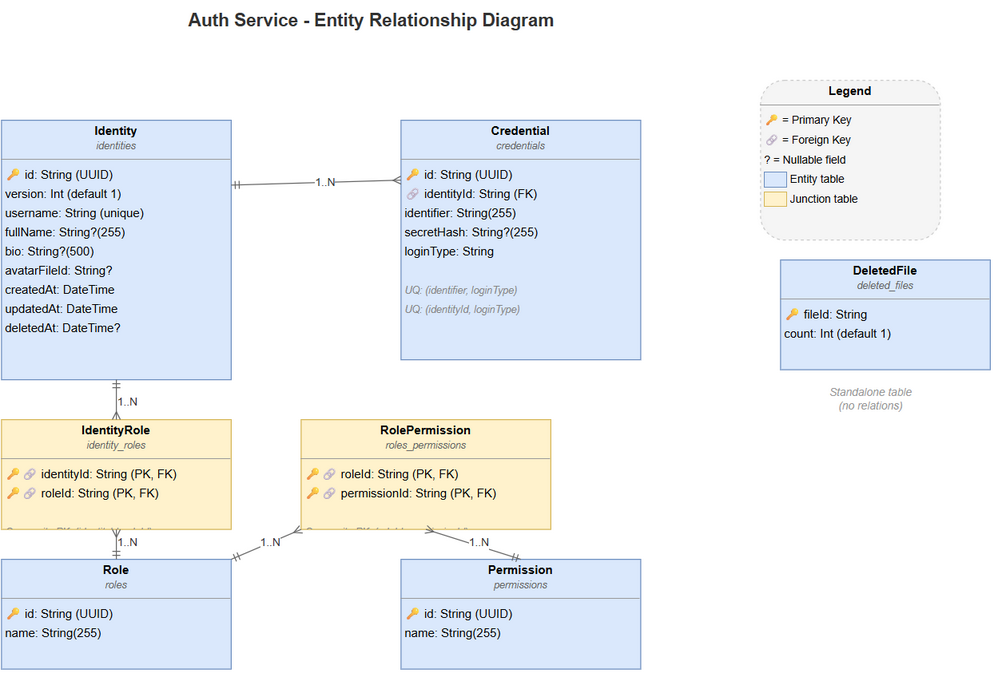
\includegraphics[width=\linewidth]{graphics/db/erd_auth}
        \captionsetup{skip=5pt}
        \caption{ERD --- Auth Service (Identity, Credential, RBAC)}
        \label{ERDAuth}
\end{figure}

Auth Service quản lý danh tính người dùng và phân quyền. Các thực thể chính:
\begin{itemize}
    \item \textbf{Identity}: Danh tính người dùng (username, fullName, bio, avatar). Hỗ trợ soft-delete qua trường \texttt{deletedAt}.
    \item \textbf{Credential}: Thông tin xác thực (identifier, secretHash, loginType). Một Identity có thể có nhiều Credential (email + Google OAuth).
    \item \textbf{Role} và \textbf{Permission}: Hệ thống RBAC thông qua hai bảng trung gian \texttt{IdentityRole} và \texttt{RolePermission}.
    \item \textbf{DeletedFile}: Theo dõi file đã xóa để đồng bộ với File Service qua RabbitMQ event.
\end{itemize}

\subsection{Exam Service}
\begin{figure}[H]
        \centering
        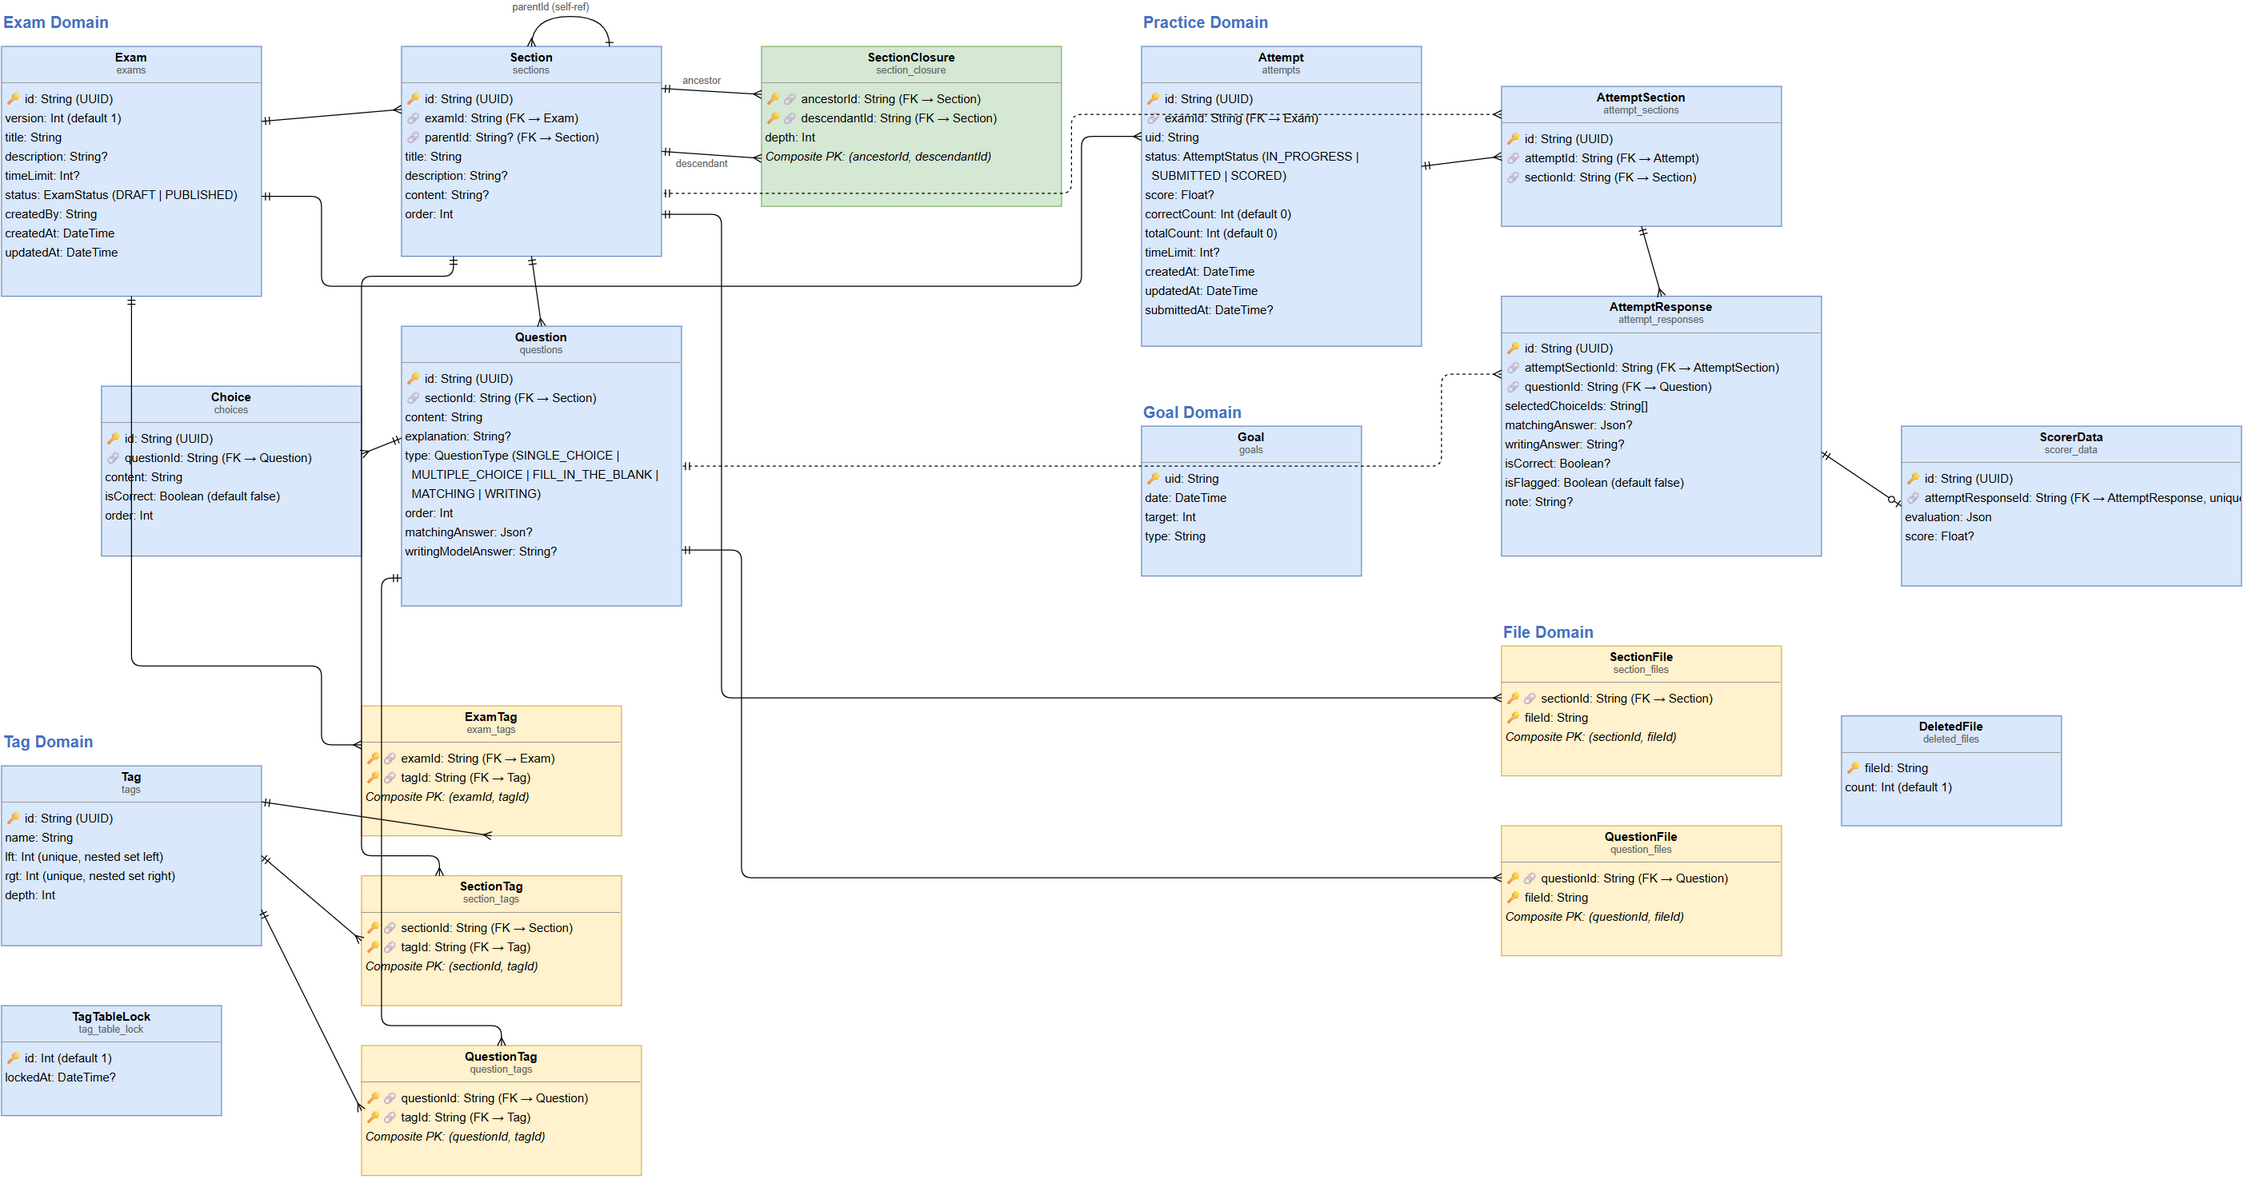
\includegraphics[width=\linewidth]{graphics/db/erd_exam}
        \captionsetup{skip=5pt}
        \caption{ERD --- Exam Service (Exam, Practice, Tag, Goal, File)}
        \label{ERDExam}
\end{figure}

Exam Service là service lớn nhất, bao gồm 18 bảng được chia thành 5 domain:

\subsubsection{Exam Domain}
\begin{itemize}
    \item \textbf{Exam}: Bài thi với lifecycle DRAFT → PUBLISHED. Chứa title, description, timeLimit và createdBy.
    \item \textbf{Section}: Các phần thi, hỗ trợ lồng nhau (self-referential qua parentId). Sử dụng \textbf{Closure Table} (\texttt{SectionClosure}) để truy vấn cây hiệu quả.
    \item \textbf{Question}: Câu hỏi với 5 loại (SINGLE\_CHOICE, MULTIPLE\_CHOICE, FILL\_IN\_THE\_BLANK, MATCHING, WRITING).
    \item \textbf{Choice}: Đáp án cho câu hỏi trắc nghiệm.
\end{itemize}

\subsubsection{Practice Domain}
\begin{itemize}
    \item \textbf{Attempt}: Lần làm bài với lifecycle IN\_PROGRESS → SUBMITTED → SCORED.
    \item \textbf{AttemptSection}: Liên kết attempt với section cụ thể.
    \item \textbf{AttemptResponse}: Câu trả lời của người dùng, hỗ trợ flag và ghi chú cá nhân.
    \item \textbf{ScorerData}: Kết quả chấm điểm AI cho bài Writing (JSON evaluation).
\end{itemize}

\subsubsection{Tag Domain}
\begin{itemize}
    \item \textbf{Tag}: Hệ thống phân loại dạng cây sử dụng \textbf{Nested Set Model} (lft/rgt) cho truy vấn subtree hiệu quả.
    \item \textbf{ExamTag}, \textbf{SectionTag}, \textbf{QuestionTag}: Bảng trung gian liên kết tag với các thực thể.
    \item \textbf{TagTableLock}: Khóa bảng để tránh race condition khi cập nhật giá trị lft/rgt.
\end{itemize}

\subsubsection{File \& Goal Domain}
\begin{itemize}
    \item \textbf{SectionFile}, \textbf{QuestionFile}: Liên kết file đính kèm với section/question.
    \item \textbf{Goal}: Mục tiêu luyện tập cá nhân (uid là PK --- mỗi người dùng một goal).
\end{itemize}

\subsection{Achievement Service}
\begin{figure}[H]
        \centering
        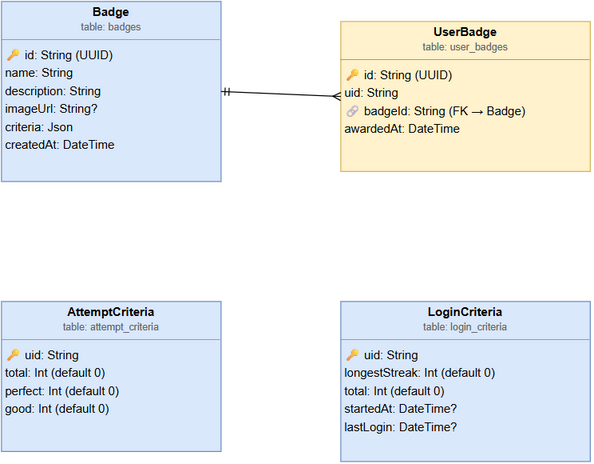
\includegraphics[width=0.8\linewidth]{graphics/db/erd_achievement}
        \captionsetup{skip=5pt}
        \caption{ERD --- Achievement Service (Badges, Criteria)}
        \label{ERDAchievement}
\end{figure}

Achievement Service quản lý hệ thống huy hiệu event-driven:
\begin{itemize}
    \item \textbf{Badge}: Định nghĩa huy hiệu (name, description, imageUrl, criteria dạng JSON).
    \item \textbf{UserBadge}: Ghi nhận huy hiệu đã được trao cho người dùng.
    \item \textbf{LoginCriteria}: Theo dõi streak đăng nhập (longestStreak, total, lastLogin).
    \item \textbf{AttemptCriteria}: Theo dõi số lần làm bài (total, perfect, good).
\end{itemize}

\subsection{File Service}
\begin{figure}[H]
        \centering
        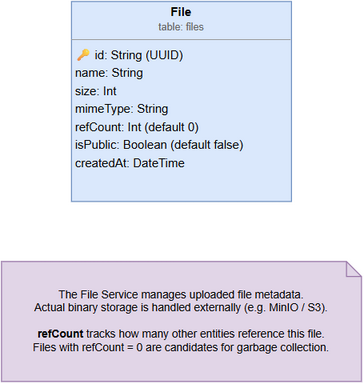
\includegraphics[width=0.5\linewidth]{graphics/db/erd_file_service}
        \captionsetup{skip=5pt}
        \caption{ERD --- File Service}
        \label{ERDFile}
\end{figure}

File Service chỉ có một bảng \textbf{File} với các trường: name, size, mimeType, refCount (đếm số lần tham chiếu), isPublic. Khi refCount về 0, file được đánh dấu là orphan và sẽ bị xóa bởi BullMQ scheduled job.

\subsection{Live Chat Service (chưa merge)}
\begin{figure}[H]
        \centering
        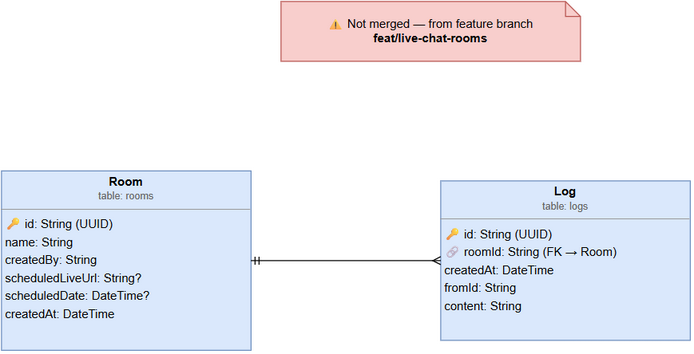
\includegraphics[width=0.7\linewidth]{graphics/db/erd_live}
        \captionsetup{skip=5pt}
        \caption{ERD --- Live Chat Service (branch \texttt{feat/live-chat-rooms})}
        \label{ERDLive}
\end{figure}

Live Chat Service (trên branch \texttt{feat/live-chat-rooms}, chưa merge vào main) bao gồm:
\begin{itemize}
    \item \textbf{Room}: Phòng chat với name, createdBy, scheduledLiveUrl và scheduledDate.
    \item \textbf{Log}: Tin nhắn trong phòng chat, liên kết với Room qua roomId.
\end{itemize}

\subsection{Resource Service (chưa merge)}
\begin{figure}[H]
        \centering
        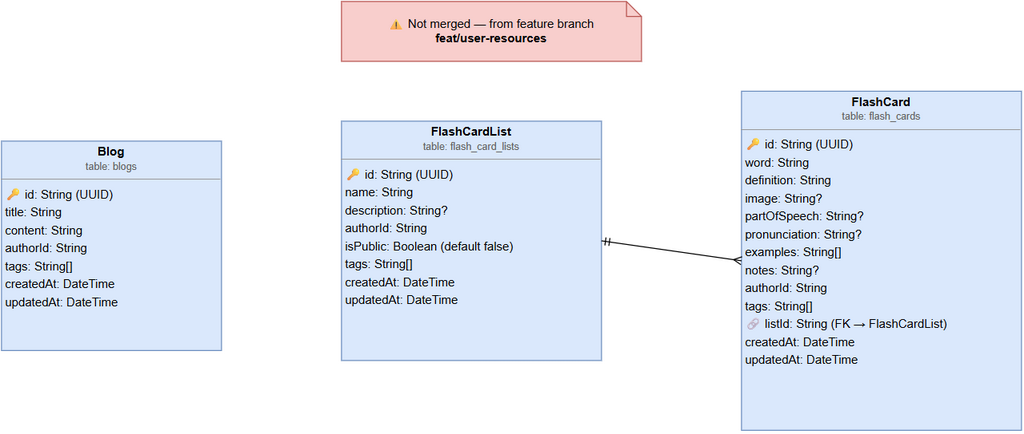
\includegraphics[width=0.8\linewidth]{graphics/db/erd_resource}
        \captionsetup{skip=5pt}
        \caption{ERD --- Resource Service (branch \texttt{feat/user-resources})}
        \label{ERDResource}
\end{figure}

Resource Service (trên branch \texttt{feat/user-resources}, chưa merge vào main) bao gồm:
\begin{itemize}
    \item \textbf{Blog}: Bài viết với title, content, authorId và tags (mảng String).
    \item \textbf{FlashCardList}: Bộ flashcard với name, description, isPublic và tags.
    \item \textbf{FlashCard}: Thẻ từ vựng với word, definition, pronunciation, examples, liên kết với FlashCardList qua listId.
\end{itemize}

\subsection{Engapp-v2 (Monolith PostgreSQL)}
\begin{figure}[H]
        \centering
        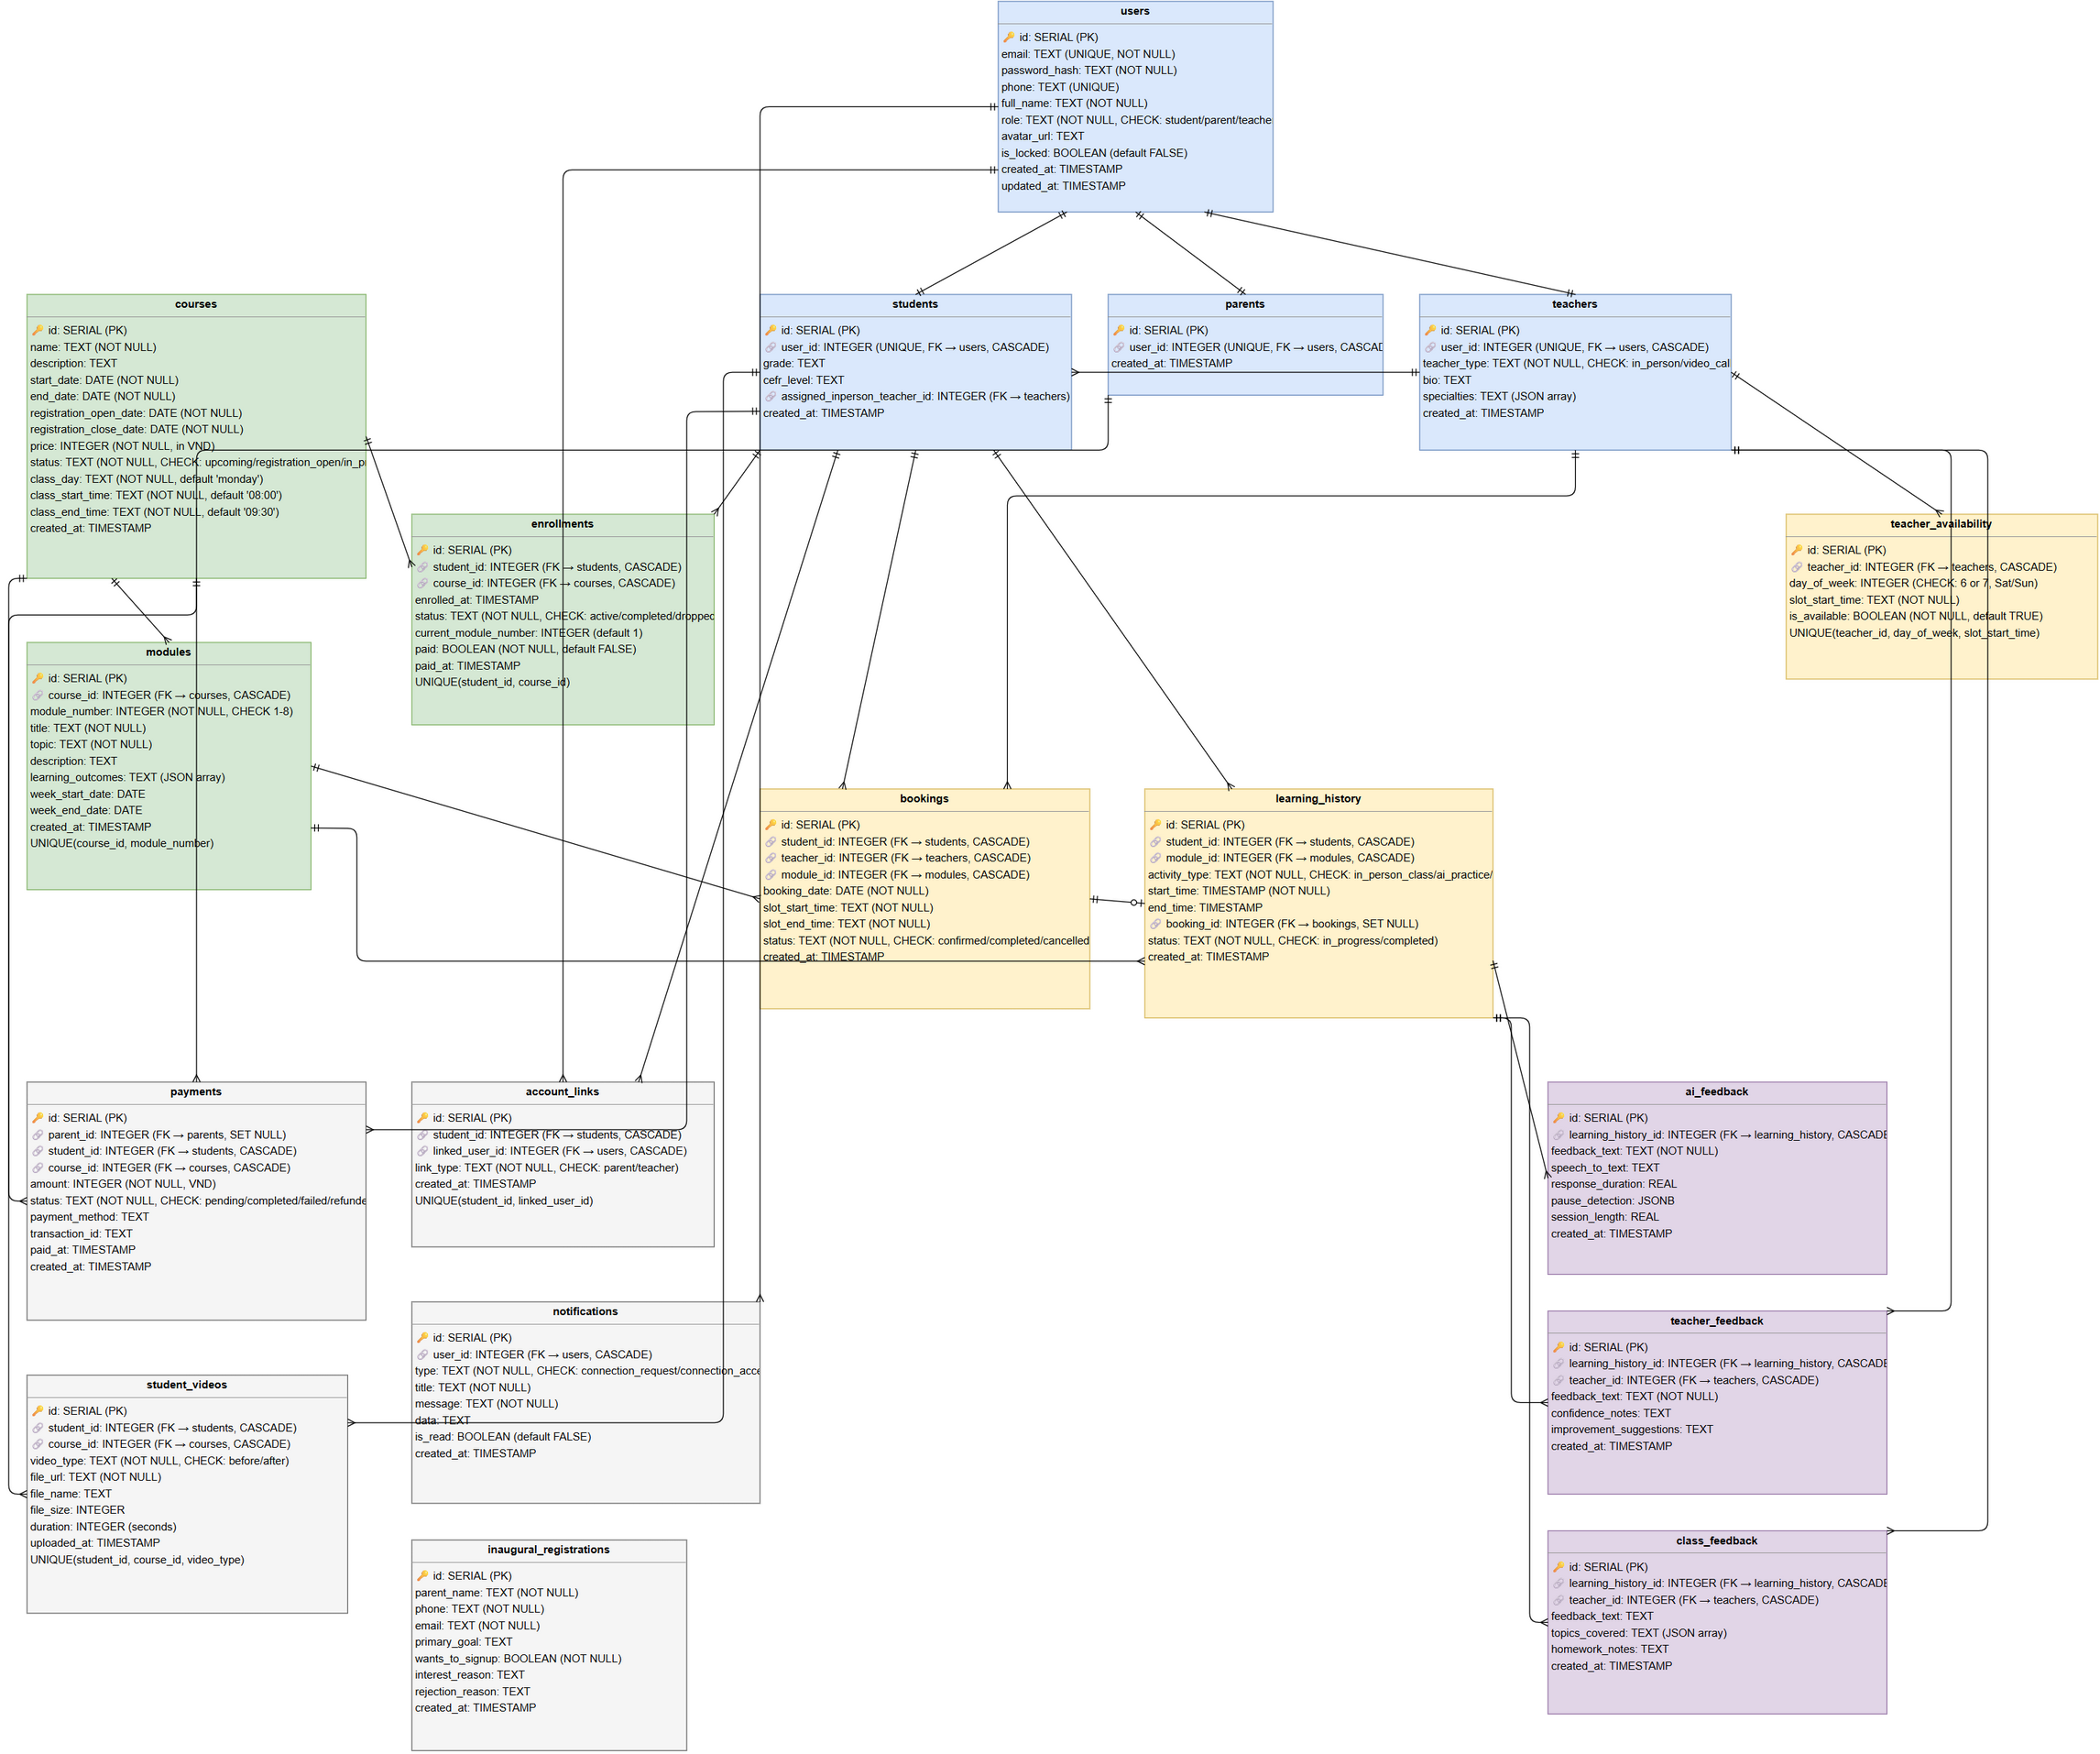
\includegraphics[width=\linewidth]{graphics/db/erd_engapp_v2}
        \captionsetup{skip=5pt}
        \caption{ERD --- Nền tảng Engapp-v2 (PostgreSQL trên Neon)}
        \label{ERDEngapp}
\end{figure}

Nền tảng Engapp-v2 sử dụng một cơ sở dữ liệu PostgreSQL duy nhất (trên Neon) với 18 bảng, chia thành các nhóm chính:
\begin{itemize}
    \item \textbf{Users \& Roles}: \texttt{users} (bảng gốc), \texttt{students}, \texttt{parents}, \texttt{teachers} (bảng mở rộng theo role), \texttt{account\_links} (liên kết tài khoản).
    \item \textbf{Course \& Enrollment}: \texttt{courses} (khóa học 8 module), \texttt{modules} (8 tuần/khóa), \texttt{enrollments} (ghi danh kèm trạng thái thanh toán).
    \item \textbf{Booking}: \texttt{teacher\_availability} (lịch dạy cuối tuần), \texttt{bookings} (lịch video call).
    \item \textbf{Learning History \& Feedback}: \texttt{learning\_history} (ghi nhận mọi hoạt động học), \texttt{ai\_feedback} (phản hồi từ AI), \texttt{teacher\_feedback} (phản hồi từ giáo viên), \texttt{class\_feedback} (phản hồi từ lớp trực tiếp).
    \item \textbf{Khác}: \texttt{payments} (thanh toán SePay), \texttt{student\_videos} (video trước/sau khóa), \texttt{notifications}, \texttt{inaugural\_registrations} (form đăng ký quan tâm).
\end{itemize}

\subsection{Giải pháp cho dữ liệu phân cấp}
\subsubsection{Các vấn đề}
Trong quá trình hiện thực prototype, chúng tôi nhận ra rằng trong Exam Service và shared Tag kernel, việc lưu trữ comments, tags và exams --- vốn bao gồm nested sections (đối với exam), nested tags và nested reply chain (đối với comment) --- cần sử dụng một cấu trúc phân cấp hoặc quan hệ phù hợp. Nếu không mô hình hóa đúng các nested relationship, những query dùng để truy xuất exam cùng section và comment tương ứng rất dễ phát sinh vấn đề N+1 query, dẫn đến truy cập cơ sở dữ liệu kém hiệu quả và tạo ra performance bottleneck.
\subsubsection{Các giải pháp}
Chúng tôi xác định hai hướng giải quyết khả thi: Nested Set Model và Closure Table \cite{closure_table}.

\textbf{Nested Set Model}
Nested Set Model là một cách biểu diễn dữ liệu phân cấp trong một bảng duy nhất bằng cách sử dụng giá trị trái và phải cho mỗi nút. Cách tiếp cận này cho phép truy xuất cây con và duyệt cấu trúc phân cấp một cách hiệu quả.

\begin{itemize}
  \item \textbf{Ưu điểm:}
  \begin{itemize}
      \item Hiệu quả đối với các thao tác read-heavy, chẳng hạn như truy xuất toàn bộ subtree chỉ bằng một query.
      \item Biểu diễn cấu trúc phân cấp đơn giản trong một bảng duy nhất.
      \item Phù hợp cho reporting hoặc tree traversal khi cấu trúc phân cấp ít thay đổi.
  \end{itemize}

  \item \textbf{Nhược điểm:}
  \begin{itemize}
      \item Các thao tác insertion, deletion hoặc di chuyển đều yêu cầu cập nhật nhiều node, khiến chi phí thay đổi cao.
      \item Khó maintain nếu cây thay đổi thường xuyên.
      \item Phức tạp hơn trong việc hiểu và triển khai so với adjacency list đơn giản.
  \end{itemize}
\end{itemize}

\textbf{Closure Table}
Cách tiếp cận Closure Table sử dụng một bảng phụ để lưu toàn bộ quan hệ tổ tiên - hậu duệ. Điều này cho phép quản lý dữ liệu phân cấp một cách linh hoạt và hiệu quả.

\begin{itemize}
  \item \textbf{Ưu điểm:}
  \begin{itemize}
      \item Xử lý tốt các cấu trúc phân cấp động; việc thêm, xóa hoặc di chuyển node tương đối dễ dàng.
      \item Các query truy tìm ancestor, descendant hoặc độ dài đường đi đều đơn giản và nhanh.
      \item Hỗ trợ tốt nhiều cấu trúc phân cấp hoặc directed acyclic graph (DAG).
  \end{itemize}

  \item \textbf{Nhược điểm:}
  \begin{itemize}
      \item Yêu cầu thêm một bảng phụ để lưu toàn bộ quan hệ ancestor-descendant.
      \item Tốn thêm storage overhead so với Nested Set Model.
      \item Có thể chậm hơn với các cây quá sâu nếu index không được áp dụng hợp lý.
  \end{itemize}
\end{itemize}